%CLASSE DOCUMENTO - LINGUA E DIMENSIONE FONT
\documentclass[11pt]{toptesi}

%%%%%%%%%%%%%%%%%%%%%%%%%%%%%%%%%%%%%%%%%%%%%%%%%%%%%%%%%%%%%%%

% INCLUSIONE PACCHETTI
		
%s\usepackage{fullpage}	
\usepackage{graphicx}
\usepackage[pagestyles]{titlesec}
\usepackage[flushleft]{caption}
\usepackage{setspace}
\usepackage[utf8]{inputenc} %utf8 % lettere accentate da tastiera
\usepackage[italian]{babel} % lingua del documento
\usepackage[T1]{fontenc} % codifica dei font
\usepackage{blindtext}
\usepackage{graphicx,wrapfig}
\usepackage{booktabs}
\usepackage[table,xcdraw]{xcolor}
\usepackage{lmodern}
\usepackage{varioref}
\usepackage{url}
\usepackage{array}
\usepackage{paralist}{\obeyspaces\global\let =\space}
\usepackage{verbatim} 
\usepackage{subfig}
\usepackage{tabularx}
\usepackage{amsmath}
\usepackage{amsfonts}
\usepackage{float}
\usepackage{amssymb}
\usepackage{multicol}
\usepackage{color}
\usepackage{multirow}
\usepackage{listings}
\usepackage[pass]{geometry}
\usepackage[figuresright]{rotating}
\usepackage{algorithm}
\usepackage{algorithmic}
\usepackage{amsmath}
\usepackage[babel]{csquotes}
\usepackage{hyperref}
\usepackage[backend=bibtex,sorting=none]{biblatex}
\usepackage{array}
\usepackage{nameref}
%\newcommand{\cellavuota}{\multicolumn{1}{c|}{}}
%\newcommand{\centra}[1]{\begin{center}#1\end{center}   }

\newcommand{\setfont}[1]{\fontfamily{iwona}\selectfont \scshape #1}
%%%%%%%%%%%%%%%%%%%%%%%%%%%%%%%%%%%%%%%%%%%%%%%%%%%%%%%%%%%%%%%

% CONFIGURAZIONE LINK E RIFERIMENTI
\hypersetup{%
    pdfpagemode={UseOutlines},
    bookmarksopen,
    pdfstartview={FitH},
    colorlinks,
    linkcolor={black}, %COLORE DEI RIFERIMENTI AL TESTO
    citecolor={blue}, %COLORE DEI RIFERIMENTI ALLE CITAZIONI
    urlcolor={blue} %COLORI DEGLI URL
}

%%%%%%%%%%%%%%%%%%%%%%%%%%%%%%%%%%%%%%%%%%%%%%%%%%%%%%%%%%%%%%%

% CONFIGURAZIONE LISTATI/CODICE - CANCELLARE SE NON NECESSARIO
% PYTHON - BIANCO E NERO
\lstset{%
	captionpos=b,
	language=Python,
	basicstyle =\small\ttfamily,
	keywordstyle=\color{black}\bfseries,
	breaklines=true,
	breakatwhitespace=true,
	frame=lines,
	numbers=left,
	numberstyle=\footnotesize,
}

%%%%%%%%%%%%%%%%%%%%%%%%%%%%%%%%%%%%%%%%%%%%%%%%%%%%%%%%%%%%%%%

% FRENCHSPACING VA _SEMPRE_ ABILITATO PER DOCUMENTI IN ITALIANO
\frenchspacing

%%%%%%%%%%%%%%%%%%%%%%%%%%%%%%%%%%%%%%%%%%%%%%%%%%%%%%%%%%%%%%%

%DEFINIZIONE SEZIONI IN NUMERAZIONE ROMANA
%ELENCO DEI LISTATI/CODICI
\makeatletter
\newcommand\listofcodes{%
 \iffrontmatter\else\frontmattertrue\fi
 \if@openright\cleardoublepage\else\clearpage\fi
 % change the meaning of \chapter in a group
 \begingroup\def\chapter##1{\@schapter}
 \phantomsection % for the hyperlink
 \lstlistoflistings 
 \endgroup
} 
\makeatother

%%%%%%%%%%%%%%%%%%%%%%%%%%%%%%%%%%%%%%%%%%%%%%%%%%%%%%%%%%%%%%%

% INFORMAZIONI PDF - PERSONALIZZARE
\pdfinfo{%
  /Title    (Reti neutrali per l’apprendimento dei tratti della personalità dal linguaggio naturale)
  /Author   (Giorgia Adorni)
  /Subject  (Laura Informatica)
  /Keywords (Tesi)
}

%%%%%%%%%%%%%%%%%%%%%%%%%%%%%%%%%%%%%%%%%%%%%%%%%%%%%%%%%%%%%%%


% LISTA DEI CAPITOLI DA INCLUDERE - PERSONALIZZARE
\includeonly{%
frontespizio,%
abstract,%
introduzione,%
contesto, %
neural_network,%
formulazione,
esperimenti,
conclusioni,
chap_quo,%
chap_qua,%
app_a,%
}

%%%%%%%%%%%%%%%%%%%%%%%%%%%%%%%%%%%%%%%%%%%%%%%%%%%%%%%%%%%%%%%


% FILE DI BIBLIOGRAFIA
\bibliography{bibliography} 

% INIZIO DOCUMENTO
\begin{document}
	
% FRONTESPIZIO
\newpage
\pagestyle{empty} % no number
\noindent

\begin{figure}\doublespacing
	\mbox{
				\begin{minipage}{.20\textwidth}
					\includegraphics[height=3.3cm]{images/LogoBicocca.pdf}
				\end{minipage}%
				\quad\quad
				\begin{minipage}[c]{.90\textwidth}
					{Università degli Studi Milano Bicocca}\\
					{  \textbf{Scuola di Scienze}}\\
					{\textbf{Dipartimento di Informatica, Sistemistica e Comunicazione}}\\
					{  \textbf{Corso di Laurea in Informatica}}
				\end{minipage}%
	}

\end{figure}

\begin{center}
	\vspace{35mm}
\doublespacing\textbf{\huge RETI NEURALI PER~L’APPRENDIMENTO DEI TRATTI DELLA PERSONALITÀ DAL LINGUAGGIO NATURALE }\\
	
\end{center}

\vspace{30mm}
\onehalfspacing 

\begin{tabular}{ll}
	\textbf{Relatore: } & {Prof. Stella Fabio Antonio}\\
	\textbf{Co-relatore: } & {Dott. Marelli Marco}
\end{tabular}

\vspace{5mm}

\begin{flushright}\onehalfspacing 
	\textbf{Relazione della prova finale di:}\\
	{Giorgia Adorni}\\
	{Matricola 806787}\end{flushright}

\vspace{25mm}
\begin{center} \textbf{Anno Accademico 2017-2018 }\end{center}


%%%%%%%%%%%%%%%%%%%%%%%%%%%%%%%%%%%%%%%%%%%%%%%%%%%%%%%%%%%%%%%

%INTERLINEA - DEFAULT 1 - NON ESAGERATE, NON SUPERATE MAI 1.3 ;)
%\interlinea{1.2}

%%%%%%%%%%%%%%%%%%%%%%%%%%%%%%%%%%%%%%%%%%%%%%%%%%%%%%%%%%%%%%%
\frontmatter

% DEDICA
% VSPACE - PROPORZIONE USATA PER CENTRATURA VERTICALE DEL TESTO
% FLUSHRIGHT - ALLINEAMENTO ORIZZONTALE A DESTRA
\vspace*{\stretch{1}}
\begin{flushright}
\noindent
\textit{A mio padre. }\\
\textit{Al mio fidanzato e collega. }
\end{flushright}
\vspace*{\stretch{6}}
\cleardoublepage


% CITAZIONE 
% VSPACE - PROPORZIONE USATA PER CENTRATURA VERTICALE DEL TESTO
% FLUSHRIGHT - ALLINEAMENTO ORIZZONTALE A DESTRA
\vspace*{\stretch{1}}
\begin{flushright}
\noindent
Citatemi dicendo che sono stato citato male.
\textit{Groucho Marx}
\end{flushright}

\vspace*{\stretch{6}}
\cleardoublepage

%%%%%%%%%%%%%%%%%%%%%%%%%%%%%%%%%%%%%%%%%%%%%%%%%%%%%%%%%%%%%%%

% RINGRAZIAMENTI - PERSONALIZZARE
\ringraziamenti
Grazie al mio relatore Fabio Stella e ai ragazzi del laboratorio MAD (Models and Algorithms for Data \& text mining).

%%%%%%%%%%%%%%%%%%%%%%%%%%%%%%%%%%%%%%%%%%%%%%%%%%%%%%%%%%%%%%%

% ABSTRACT - PERSONALIZZARE
\sommario

La personalità è considerata come uno degli argomenti di ricerca più influenti in psicologia poiché predittiva di molti esiti consequenziali come la salute mentale e fisica, ed è in grado di spiegare il comportamento umano.
Grazie alla diffusione dei Social Network come mezzo di comunicazione, sta diventando sempre più importante sviluppare modelli che possano leggere automaticamente e con precisione l'essenza di individui basandosi esclusivamente sulla scrittura. 
\\\\
In particolare la convergenza tra scienze sociali e informatiche ha portato i ricercatori a sviluppare approcci automatici per estrarre e studiare le informazioni "nascoste" nei dati testuali presenti in rete.
La natura di questo progetto di tesi è altamente sperimentale, e la motivazione alla base di questo lavoro è presentare delle analisi dettagliate sull'argomento, in quanto allo stato attuale non esistono importanti indagini di questo tipo.
\\\\
Obiettivo è identificare un adeguato spazio semantico che permetta di definire la personalità dell'oggetto a cui un determinato testo si riferisce. Punto di partenza è un dizionario di aggettivi che la letteratura psicologica definisce come marker dei cinque grandi tratti di personalità o Big Five.
\\\\
In questo lavoro siamo partiti dall'implementazione di reti neurali  fully-connected come base per capire come i modelli semplici in deep-learning possano fornire informazioni sulle caratteristiche della personalità nascoste. 
\\\\
Infine utilizziamo una classe di algoritmi distribuzionali inventati nel 2013 da \emph{Tomas Mikolov}, che consistono nell'utilizzo di una rete neurale convoluzionale, che impara in modo non supervisionato i contesti delle parole.
In questo modo costruiamo un embedding in cui sono contenute le informazioni semantiche del testo, ottenendo una sorta di “geometria del significato” in cui i concetti sono tradotti in relazioni lineari.
Con quest'ultimo esperimento ipotizziamo che uno stile di scrittura individuale sia in gran parte accoppiato con i tratti della sua personalità.

%%%%%%%%%%%%%%%%%%%%%%%%%%%%%%%%%%%%%%%%%%%%%%%%%%%%%%%%%%%%%%%
% INDICI 

% INDICE GENERALE
\tableofcontents

% INDICE DELLE FIGURE
\listoffigures

% INDICE DELLE TABELLE
\listoftables

% INDICE DEI CODICI
\listofcodes

%%%%%%%%%%%%%%%%%%%%%%%%%%%%%%%%%%%%%%%%%%%%%%%%%%%%%%%%%%%%%%%
\introduzione
\chapter{Introduzione}
\label{chap:introduzione}
\Blindtext

Data mining: estrazione di significato da grandi quantità di dati
analisi dell'espressione umana che rendo conto da una parte del linguaggio come veicolo di definizione e di affermazione del se
evoluzione della comunicazione verso le nuove forme di dialogo tra persone e comunità

la raccolta di dadi e la necessità di produrre analisi sempre più velocemente ha fatto crescere in questa direzione la ricerca nel campo dell'apprendimento automatico o \emph{machine learning}.
In particolare, nell'ambito del text mining, si sono sviluppate metodologie che consentono ai computer di confrontarsi con il linguaggio umano, di elaborarlo e comprenderlo.


L'obiettivo di questa tesi è descrivere e sfruttare alcune tecniche come il machine learning e Natural Language Processing nell'ambito del ... 


Extroversion was the strongest predictor of leadership emergence — who becomes a leader — and leadership effectiveness — who's successful in a leadership position. But it was a better predictor of emergence than effectiveness.

What's more, when the study authors deconstructed extroversion into distinct parts, they found that dominance and sociability better predicted leadership than extroversion as a whole. This makes sense, the study authors write, "as both sociable and dominant people are more likely to assert themselves in group situations."
Conscientiousness, or a person's tendency to be organized and hard-working, was the second strongest predictor of leadership.
Again, conscientiousness was more closely linked to leader emergence than to leadership effectiveness. The authors write: "[T]he organizing activities of conscientious individuals (e.g. note taking, facilitating processes) may allow such individuals to quickly emerge as leaders.

In business settings, openness to experience is an important predictor of leadership. Justin Sullivan / Getty
Openness to experience was the third strongest predictor of leadership. However, it's worth noting that, in business settings specifically, openness was just as strongly linked to leadership as extroversion.
Neuroticism was not a strong predictor of leadership, meaning that highly neurotic people are not especially likely or unlikely to become leaders.
Agreeableness, or friendliness, was the "least relevant" to leadership of all the traits studied. Interestingly, however, when the researchers looked only at leadership effectiveness, agreeableness was related.




Psicologia e informatica:
I modelli computazionali possono essere utilizzati per modellare i sistemi come una scatola nera, ma possono anche essere usati per informare i modelli di elaborazione delle informazioni che mirano a comprendere la cognizione umana.




Le regioni cerebrali che codificano per vari tratti di personalità sono spesso accoppiate con regioni responsabili della comunicazione verbale e scritta. Inoltre, l'avvento dei social media e una comunità online sempre più connessa rendono sempre più disponibili i dati testuali personalizzati. In questo studio, ipotizziamo che uno stile di scrittura individuale è in gran parte accoppiato con i tratti della sua personalità e presenta un modello di apprendimento profondo per predire il tipo di personalità di Myers Briggs attraverso i dati testuali dei libri. Sviluppare un modello accurato e aprire questa domanda di ricerca avrebbe implicazioni significative nella business intelligence, nell'analisi della compatibilità delle relazioni e in altri campi della sociologia.










\chapter*{Abstract}
\label{Abstract}


Apprendimento della personalità basato sul linguaggio naturale. 
Reti neurali per la previsione dei tipi di personalità di Myers Brigg dagli stili di scrittura.






La personalità è l'essenza che definisce un individuo in quanto guida il modo in cui pensiamo, agiamo e interpretiamo stimoli esterni. 
Nel corso del secolo scorso, gli aspetti della personalità sono stati studiati da molti punti di vista, sia attraverso l'analisi delle relazioni interpersonali, delle dinamiche di gruppo e dei social network, sia attraverso le opere nelle neuroscienze che rivelano le basi biologiche dei tratti della personalità.


Il testo e la scrittura sono diventati un mezzo di comunicazione importante nell'era digitale. L'uso crescente dei social media e il fenomeno delle recensioni online hanno favorito un rapido aumento dei dati testuali digitali su cui vengono effettuate svariati tipi di analisi.
In particolare la convergenza tra scienze sociali (psicologiche) e informatiche hanno portato i ricercatori a sviluppare metodi automatizzati (approcci automatici) per estrarre e studiare le informazioni digitali contenute nel materiale testuale per prevedere i tratti della personalità.
La maggior parte degli attuali studi automatici di rilevamento della personalità si sono concentrati sul modello di personalità Big 5 come quadro per studiare le caratteristiche intrinseche dell'essere umano. 


Partendo da un dizionario di aggettivi che la letteratura psicologica definisce come marker dei cinque grandi tratti di personalità (Big Five), si vuole identificare un adeguato spazio semantico che permetta di definire la personalità dell’oggetto target a cui un determinato testo si riferisce. I dati che verranno utilizzati per definire lo spazio semantico e testare la sua funzionalità sono messi a disposizione da Yelp Dataset Challenge, che contiene 5˙200˙000 reviews relative a 174˙000 businesses di 11 aree metropolitane nel mondo. 




Obiettivo è la progettazione e lo sviluppo di un modello computazionale per l'apprendimento della personalità a partire dal linguaggio naturale.  


In questo studio, ipotizziamo che uno stile di scrittura individuale è in gran parte accoppiato con i tratti della sua personalità e presenta un modello di apprendimento profondo per predire il tipo di personalità di Myers Briggs attraverso i dati testuali dei libri. Sviluppare un modello accurato e aprire questa domanda di ricerca avrebbe implicazioni significative nella business intelligence, nell'analisi della compatibilità delle relazioni e in altri campi della sociologia.



La personalità è considerata uno degli argomenti di ricerca più influenti in psicologia perché è predittiva di molti esiti consequenziali come la salute mentale e fisica, la qualità delle relazioni interpersonali, l'adeguamento alla carriera e la soddisfazione, le prestazioni sul posto di lavoro e il benessere generale.

È ampiamente noto che i tratti della personalità come l'extraversione, la coscienziosità e il nevroticismo sono relativamente coerenti per tutta la vita. Tuttavia, i modi in cui i nostri comportamenti sono espressi attraverso le parole e l'azione non sono sempre determinati dai tratti soggettivi della personalità e dagli impulsi da soli.

Molte decisioni importanti, le dinamiche sociali e le decisioni politiche si basano anche sulla valutazione della personalità di un individuo con il quale non si è interagito molto personalmente. 

Ma leggere solo i comportamenti di altre persone non è sufficiente per fare previsioni accurate della loro personalità. Il compito diventa ancora più difficile quando si tenta di formulare giudizi basati solo sulla comunicazione scritta. 

Poiché il mondo si basa molto più sulla comunicazione basata sul testo rispetto alle interazioni faccia a faccia, sta diventando sempre più importante sviluppare modelli che possano leggere automaticamente e con precisione l'essenza di altri individui basandosi esclusivamente sulla scrittura. 

Fortunatamente, studi in neuroscienza hanno rivelato una mappatura vicina delle regioni del cervello responsabili dei tratti della personalità come l'extraversione e il nevroticismo, nonché quelli che sono legati alla comunicazione scritta.

I precedenti modelli di previsione della personalità si sono concentrati sull'applicazione di tecniche generali di apprendimento automatico e reti neurali per predire i tratti di personalità del Big Five di openness, conscientiousness, extraversion, agreeableness e neuroticism dai post sui social media. 

Gli studi che si focalizzano sui tratti del Big Five tendono a dare un tratto alla figura di un individuo.


In questo lavoro, abbiamo esplorato una varietà di metodi per affrontare il problema della predizione della personalità. 

Abbiamo iniziato costruendo manualmente un vasto corpus di brani tratti da romanzi famosi con autori di tipi MBTI. 

Per valutare la difficoltà di identificare gli MBTI dal testo, abbiamo raggruppato segmenti di testo basati su somiglianze di incorporamento di parole per determinare se esistesse una distribuzione non uniforme di tipi di personalità. Ciò fornisce una buona cornice iniziale di riferimento per capire quanto siano sottili i tratti della personalità quando sono nascosti nei dati scritti. 

Abbiamo poi implementato un sacco di reti neurali feed-forward come base per capire come i modelli semplici in deep-learning possano fornire informazioni sulle caratteristiche della personalità nascoste. 

Infine, ci addentriamo in una rete neuronale ricorrente basata sulla memoria a lungo termine più complessa e miriamo a costruire un sistema più generalizzabile che possa incorporare il significato della scrittura per determinare i tipi di personalità generali.



tratti di personalità Big 5.

I risultati delle analisi mostrano che il potere predittivo delle impronte digitali sui tratti della personalità è in linea con il 
Nel complesso, i nostri risultati indicano che la precisione delle previsioni è coerente tra i tratti Big 5 e che l'accuratezza migliora quando le analisi includono dati demografici e diversi tipi di impronte digitali.



struttura di personalità per guidare la nostra comprensione e rivelare il ruolo delle parole nel descrivere le caratteristiche di un utente. 
Questo studio preliminare ha rivelato come le percezioni del pubblico riguardo a parole specifiche possano aiutarci a rilevare la personalità. 

Come prima fase del nostro studio, questo esperimento si concentra sulla raccolta delle percezioni generali dei malesi verso 52 aggettivi inglesi categorizzazione delle parole sotto tratti PEN. 
La valutazione fornisce l'analisi necessaria che potrebbe aiutare la nostra ricerca principale che si concentra su rilevazioni automatiche della personalità. 










Abbiamo iniziato costruendo manualmente un vasto corpus di brani tratti da romanzi famosi con autori di tipi MBTI. 

Per valutare la difficoltà di identificare gli MBTI dal testo, abbiamo raggruppato segmenti di testo basati su somiglianze di incorporamento di parole per determinare se esistesse una distribuzione non uniforme di tipi di personalità. Ciò fornisce una buona cornice iniziale di riferimento per capire quanto siano sottili i tratti della personalità quando sono nascosti nei dati scritti. 



I risultati delle analisi mostrano che il potere predittivo delle impronte digitali sui tratti della personalità è in linea con il 
Nel complesso, i nostri risultati indicano che la precisione delle previsioni è coerente tra i tratti Big 5 e che l'accuratezza migliora quando le analisi includono dati demografici e diversi tipi di impronte digitali.


struttura di personalità per guidare la nostra comprensione e rivelare il ruolo delle parole nel descrivere le caratteristiche di un utente. 
Questo studio preliminare ha rivelato come le percezioni del pubblico riguardo a parole specifiche possano aiutarci a rilevare la personalità. 

Come prima fase del nostro studio, questo esperimento si concentra sulla raccolta delle percezioni generali dei malesi verso 52 aggettivi inglesi categorizzazione delle parole sotto tratti PEN. 
La valutazione fornisce l'analisi necessaria che potrebbe aiutare la nostra ricerca principale che si concentra su rilevazioni automatiche della personalità. 






% INCLUSIONE FILE CAPITOLI - TENERE COERENTE CON LISTA IN ALTO

\mainmatter
%\chapter{Introduzione}
\label{chap:introduzione}
\Blindtext

Data mining: estrazione di significato da grandi quantità di dati
analisi dell'espressione umana che rendo conto da una parte del linguaggio come veicolo di definizione e di affermazione del se
evoluzione della comunicazione verso le nuove forme di dialogo tra persone e comunità

la raccolta di dadi e la necessità di produrre analisi sempre più velocemente ha fatto crescere in questa direzione la ricerca nel campo dell'apprendimento automatico o \emph{machine learning}.
In particolare, nell'ambito del text mining, si sono sviluppate metodologie che consentono ai computer di confrontarsi con il linguaggio umano, di elaborarlo e comprenderlo.


L'obiettivo di questa tesi è descrivere e sfruttare alcune tecniche come il machine learning e Natural Language Processing nell'ambito del ... 


Extroversion was the strongest predictor of leadership emergence — who becomes a leader — and leadership effectiveness — who's successful in a leadership position. But it was a better predictor of emergence than effectiveness.

What's more, when the study authors deconstructed extroversion into distinct parts, they found that dominance and sociability better predicted leadership than extroversion as a whole. This makes sense, the study authors write, "as both sociable and dominant people are more likely to assert themselves in group situations."
Conscientiousness, or a person's tendency to be organized and hard-working, was the second strongest predictor of leadership.
Again, conscientiousness was more closely linked to leader emergence than to leadership effectiveness. The authors write: "[T]he organizing activities of conscientious individuals (e.g. note taking, facilitating processes) may allow such individuals to quickly emerge as leaders.

In business settings, openness to experience is an important predictor of leadership. Justin Sullivan / Getty
Openness to experience was the third strongest predictor of leadership. However, it's worth noting that, in business settings specifically, openness was just as strongly linked to leadership as extroversion.
Neuroticism was not a strong predictor of leadership, meaning that highly neurotic people are not especially likely or unlikely to become leaders.
Agreeableness, or friendliness, was the "least relevant" to leadership of all the traits studied. Interestingly, however, when the researchers looked only at leadership effectiveness, agreeableness was related.




Psicologia e informatica:
I modelli computazionali possono essere utilizzati per modellare i sistemi come una scatola nera, ma possono anche essere usati per informare i modelli di elaborazione delle informazioni che mirano a comprendere la cognizione umana.




Le regioni cerebrali che codificano per vari tratti di personalità sono spesso accoppiate con regioni responsabili della comunicazione verbale e scritta. Inoltre, l'avvento dei social media e una comunità online sempre più connessa rendono sempre più disponibili i dati testuali personalizzati. In questo studio, ipotizziamo che uno stile di scrittura individuale è in gran parte accoppiato con i tratti della sua personalità e presenta un modello di apprendimento profondo per predire il tipo di personalità di Myers Briggs attraverso i dati testuali dei libri. Sviluppare un modello accurato e aprire questa domanda di ricerca avrebbe implicazioni significative nella business intelligence, nell'analisi della compatibilità delle relazioni e in altri campi della sociologia.










\chapter*{Abstract}
\label{Abstract}


Apprendimento della personalità basato sul linguaggio naturale. 
Reti neurali per la previsione dei tipi di personalità di Myers Brigg dagli stili di scrittura.






La personalità è l'essenza che definisce un individuo in quanto guida il modo in cui pensiamo, agiamo e interpretiamo stimoli esterni. 
Nel corso del secolo scorso, gli aspetti della personalità sono stati studiati da molti punti di vista, sia attraverso l'analisi delle relazioni interpersonali, delle dinamiche di gruppo e dei social network, sia attraverso le opere nelle neuroscienze che rivelano le basi biologiche dei tratti della personalità.


Il testo e la scrittura sono diventati un mezzo di comunicazione importante nell'era digitale. L'uso crescente dei social media e il fenomeno delle recensioni online hanno favorito un rapido aumento dei dati testuali digitali su cui vengono effettuate svariati tipi di analisi.
In particolare la convergenza tra scienze sociali (psicologiche) e informatiche hanno portato i ricercatori a sviluppare metodi automatizzati (approcci automatici) per estrarre e studiare le informazioni digitali contenute nel materiale testuale per prevedere i tratti della personalità.
La maggior parte degli attuali studi automatici di rilevamento della personalità si sono concentrati sul modello di personalità Big 5 come quadro per studiare le caratteristiche intrinseche dell'essere umano. 


Partendo da un dizionario di aggettivi che la letteratura psicologica definisce come marker dei cinque grandi tratti di personalità (Big Five), si vuole identificare un adeguato spazio semantico che permetta di definire la personalità dell’oggetto target a cui un determinato testo si riferisce. I dati che verranno utilizzati per definire lo spazio semantico e testare la sua funzionalità sono messi a disposizione da Yelp Dataset Challenge, che contiene 5˙200˙000 reviews relative a 174˙000 businesses di 11 aree metropolitane nel mondo. 




Obiettivo è la progettazione e lo sviluppo di un modello computazionale per l'apprendimento della personalità a partire dal linguaggio naturale.  


In questo studio, ipotizziamo che uno stile di scrittura individuale è in gran parte accoppiato con i tratti della sua personalità e presenta un modello di apprendimento profondo per predire il tipo di personalità di Myers Briggs attraverso i dati testuali dei libri. Sviluppare un modello accurato e aprire questa domanda di ricerca avrebbe implicazioni significative nella business intelligence, nell'analisi della compatibilità delle relazioni e in altri campi della sociologia.



La personalità è considerata uno degli argomenti di ricerca più influenti in psicologia perché è predittiva di molti esiti consequenziali come la salute mentale e fisica, la qualità delle relazioni interpersonali, l'adeguamento alla carriera e la soddisfazione, le prestazioni sul posto di lavoro e il benessere generale.

È ampiamente noto che i tratti della personalità come l'extraversione, la coscienziosità e il nevroticismo sono relativamente coerenti per tutta la vita. Tuttavia, i modi in cui i nostri comportamenti sono espressi attraverso le parole e l'azione non sono sempre determinati dai tratti soggettivi della personalità e dagli impulsi da soli.

Molte decisioni importanti, le dinamiche sociali e le decisioni politiche si basano anche sulla valutazione della personalità di un individuo con il quale non si è interagito molto personalmente. 

Ma leggere solo i comportamenti di altre persone non è sufficiente per fare previsioni accurate della loro personalità. Il compito diventa ancora più difficile quando si tenta di formulare giudizi basati solo sulla comunicazione scritta. 

Poiché il mondo si basa molto più sulla comunicazione basata sul testo rispetto alle interazioni faccia a faccia, sta diventando sempre più importante sviluppare modelli che possano leggere automaticamente e con precisione l'essenza di altri individui basandosi esclusivamente sulla scrittura. 

Fortunatamente, studi in neuroscienza hanno rivelato una mappatura vicina delle regioni del cervello responsabili dei tratti della personalità come l'extraversione e il nevroticismo, nonché quelli che sono legati alla comunicazione scritta.

I precedenti modelli di previsione della personalità si sono concentrati sull'applicazione di tecniche generali di apprendimento automatico e reti neurali per predire i tratti di personalità del Big Five di openness, conscientiousness, extraversion, agreeableness e neuroticism dai post sui social media. 

Gli studi che si focalizzano sui tratti del Big Five tendono a dare un tratto alla figura di un individuo.


In questo lavoro, abbiamo esplorato una varietà di metodi per affrontare il problema della predizione della personalità. 

Abbiamo iniziato costruendo manualmente un vasto corpus di brani tratti da romanzi famosi con autori di tipi MBTI. 

Per valutare la difficoltà di identificare gli MBTI dal testo, abbiamo raggruppato segmenti di testo basati su somiglianze di incorporamento di parole per determinare se esistesse una distribuzione non uniforme di tipi di personalità. Ciò fornisce una buona cornice iniziale di riferimento per capire quanto siano sottili i tratti della personalità quando sono nascosti nei dati scritti. 

Abbiamo poi implementato un sacco di reti neurali feed-forward come base per capire come i modelli semplici in deep-learning possano fornire informazioni sulle caratteristiche della personalità nascoste. 

Infine, ci addentriamo in una rete neuronale ricorrente basata sulla memoria a lungo termine più complessa e miriamo a costruire un sistema più generalizzabile che possa incorporare il significato della scrittura per determinare i tipi di personalità generali.



tratti di personalità Big 5.

I risultati delle analisi mostrano che il potere predittivo delle impronte digitali sui tratti della personalità è in linea con il 
Nel complesso, i nostri risultati indicano che la precisione delle previsioni è coerente tra i tratti Big 5 e che l'accuratezza migliora quando le analisi includono dati demografici e diversi tipi di impronte digitali.



struttura di personalità per guidare la nostra comprensione e rivelare il ruolo delle parole nel descrivere le caratteristiche di un utente. 
Questo studio preliminare ha rivelato come le percezioni del pubblico riguardo a parole specifiche possano aiutarci a rilevare la personalità. 

Come prima fase del nostro studio, questo esperimento si concentra sulla raccolta delle percezioni generali dei malesi verso 52 aggettivi inglesi categorizzazione delle parole sotto tratti PEN. 
La valutazione fornisce l'analisi necessaria che potrebbe aiutare la nostra ricerca principale che si concentra su rilevazioni automatiche della personalità. 










Abbiamo iniziato costruendo manualmente un vasto corpus di brani tratti da romanzi famosi con autori di tipi MBTI. 

Per valutare la difficoltà di identificare gli MBTI dal testo, abbiamo raggruppato segmenti di testo basati su somiglianze di incorporamento di parole per determinare se esistesse una distribuzione non uniforme di tipi di personalità. Ciò fornisce una buona cornice iniziale di riferimento per capire quanto siano sottili i tratti della personalità quando sono nascosti nei dati scritti. 



I risultati delle analisi mostrano che il potere predittivo delle impronte digitali sui tratti della personalità è in linea con il 
Nel complesso, i nostri risultati indicano che la precisione delle previsioni è coerente tra i tratti Big 5 e che l'accuratezza migliora quando le analisi includono dati demografici e diversi tipi di impronte digitali.


struttura di personalità per guidare la nostra comprensione e rivelare il ruolo delle parole nel descrivere le caratteristiche di un utente. 
Questo studio preliminare ha rivelato come le percezioni del pubblico riguardo a parole specifiche possano aiutarci a rilevare la personalità. 

Come prima fase del nostro studio, questo esperimento si concentra sulla raccolta delle percezioni generali dei malesi verso 52 aggettivi inglesi categorizzazione delle parole sotto tratti PEN. 
La valutazione fornisce l'analisi necessaria che potrebbe aiutare la nostra ricerca principale che si concentra su rilevazioni automatiche della personalità. 





\chapter{Contesto}
\label{chap:contesto}

Con il termine \emph{personalità} si intende l'insieme delle caratteristiche psichiche e dei comportamentali abituali (inclinazioni, interessi, passioni) che definiscono il nucleo delle differenze individuali, nella vari contesti e ambienti in cui la condotta umana si sviluppa \cite{corr2009cambridge,sadock2000comprehensive}.
\\
Ogni nucleo teorico, in psicologia, concettualizza la personalità entro modelli diversi, adoperando metodi, obiettivi e modalità d'analisi anche molto dissonanti fra loro. 
Lo studio della psicologia della personalità tenta di spiegare le tendenze che sono alla base delle differenze di comportamento. Sono stati adottati molti approcci per studiare la personalità, comprese le teorie basate sul metodo biologico, cognitivo, dell'apprendimento e dei tratti, così come sugli approcci psicodinamici e umanistici. 
\\
La tradizione di studi psicologici relativi alla personalità è una delle più rilevanti della psicologia contemporanea, un campo in cui si susseguono studi empirici, teorici e storici, tesi a comprendere la natura dell'identità personale nel contesto biologico e sociale di sviluppo. \\
Una significativa parte della psicologia delle differenze individuali, analizza e valuta la personalità attraverso test volti ad individuarne i tratti.

\section{Big five}
\label{sec:big5}

Le teorie della personalità basate sui tratti definiscono la personalità come le caratteristiche che predicono il comportamento di una persona. 
\\
La teoria dei Grandi Cinque (o Big Five) risulta essere uno dei modelli più condivisi e testati, sia a livello teorico che empirico.
McCrae e Costa identificano cinque grandi dimensioni in cui può essere suddivisa la personalità \cite{goldberg1993structure,costa2008revised}:
\begin{itemize}
	\item L'\emph{apertura all'esperienza} o "openness" (creativo / curioso vs. coerente / cauto) è intesa come attitudine per la ricerca di stimoli culturali e di pensiero esterni al proprio contesto ordinario.
	Essa riflette il grado di curiosità intellettuale, la creatività o una preferenza per la novità, può inoltre essere percepita come imprevedibilità o mancanza di concentrazione. \\ 
	Individui con un'elevata apertura perseguono l'auto-realizzazione cercando esperienze intense ed euforiche. Viceversa, coloro che hanno una bassa apertura cercano di ottenere soddisfazione attraverso la perseveranza.
	
	\item La \emph{coscienziosità} o "conscientiousness" (organizzato vs. negligente) è una tendenza caratterizzata dall'organizzazione, precisione e affidabilità, e preferisce un comportamento pianificato piuttosto che spontaneo.\\  
	Spesso l'alta coscienziosità viene percepita come testardaggine e ossessione, mentre la bassa coscienziosità è associata alla flessibilità e alla spontaneità, ma può anche apparire come mancanza di affidabilità.
		
	\item L'\emph{estroversione} o "extraversion"  (estroverso / energetico vs. solitario / riservato) è intesa come grado di entusiasmo nelle condotte che si adottano e tendenza a cercare la stimolazione in compagnia degli altri.\\ 
	L'alta estroversione è spesso percepita come una ricerca di attenzioni e prepotenza. La bassa estroversione causa una personalità riservata, riflessiva, che può essere percepita come distaccata.  
	
	\item La \emph{gradevolezza} o "agreeableness" (amichevole / compassionevole vs. sfidante / distaccato) è indicata come quantità e qualità delle relazioni interpersonali che la persona intraprende, orientate al prendersi cura ed accogliere l'altro. È una	tendenza ad essere compassionevoli e collaborativi piuttosto che sospettosi e antagonisti verso gli altri. \\
	L'alta gradevolezza è spesso vista come ingenuità o sottomissione. Le persone con scarsa gradevolezza sono spesso competitive o sfidanti, e possono essere viste come inaffidabili.

	\item Il \emph{nevroticismo} o "neuroticism" (sensibile / nervoso vs. sicuro / fiducioso), è una misura di resistenza a stress di tipo psicologico, come l'ansietà, l'instabilità e l'irritabilità, e si riferisce anche al grado di stabilità emotiva e di controllo degli impulsi.\\
	Un'alta stabilità si manifesta in una personalità stabile e calma, ma può essere vista come poco interessante e indifferente. Una bassa stabilità esprime reattività e dinamicità in individui che spesso possono essere percepiti come instabili o insicuri. 
\end{itemize}
Queste dimensioni sono state individuate a partire da studi psico-lessicali, secondo cui le cinque dimensioni corrisponderebbero alle macro-categorie più usate, nel linguaggio, per descrivere le diversità tra individui.\\
Le regioni cerebrali che codificano i vari tratti di personalità sono spesso collegate alle regioni responsabili della comunicazione verbale e scritta. \\
I Big Five sono anche in grado di catturare altre dimensioni: sono state individuate, per ogni tratto di personalità, due sottodimensioni.
La teoria dei tratti considera ad esempio introversione ed estroversione come due estremi di un'unica linea continua su cui la popolazione si distribuirà in modo gaussiano.\\
Un grande numero di prove di ricerca ha supportato il modello a cinque fattori. Le cinque dimensioni del Big Five sembrano essere interculturali, perché gli stessi cinque fattori sono stati identificati nei partecipanti in Cina, Giappone, Italia, Ungheria, Turchia e in molti altri paesi \cite{triandis2002cultural}.\\ 
Le dimensioni di Big Five predicono accuratamente il comportamento e vengono utilizzati sempre più spesso per aiutare i ricercatori a comprendere le dimensioni dei disturbi psicologici come ansia e depressione (Oldham, 2010, Saulsman \& Page, 2004)\cite{saulsman2004five}.\\
Un vantaggio dell'approccio a cinque fattori è che è parsimonioso e consente di concentrare l'attenzione solo su cinque dimensioni di base piuttosto che studiare centinaia di tratti.
%\begin{table}[]
%	\renewcommand{\arraystretch}{1.5}
%	\centering
%	\begin{tabularx}{\textwidth}{XXXX}
%		\rowcolor[HTML]{C0C0C0} 
%		Dimension & Sample items & Descriptions & Examples of behaviours predicted by trait \tabularnewline 
%		Openness & “I have a vivid imagination”; \newline “I have a rich vocabulary”; \newline“I have excellent ideas.” & A general appreciation for art, emotion, adventure, unusual ideas, imagination,   curiosity, and variety of experience & Individuals who are highly open to experience tend to have distinctive and unconventional decorations in their home. They  are also likely to have books on a wide variety of topics, a diverse music collection, and works of art on display.\tabularnewline  
%		Conscientiousness & “I am always prepared”; \newline“I am exacting in my work”; \newline “I follow a schedule.” & A tendency to show self-discipline, act  dutifully, and aim for achievement & Individuals who are conscientious have a preference for planned rather than spontaneous behaviour. \tabularnewline 
%		Extraversion & “I am the life of the party”;\newline“I feel comfortable around people”;  \newline “I talk to a lot of different people at parties.” & The tendency to experience positive emotions and to seek out stimulation and the company of  others & Extroverts enjoy being with people. In groups they like to talk, assert themselves, and draw attention to themselves. \tabularnewline 
%		Agreeableness & “I am interested in people”; \newline “I feel others’ emotions”; \newline “I make people feel at ease.” & A tendency to be compassionate and  cooperative rather than suspicious and  antagonistic toward others; reflects individual   differences in general concern for social  harmony & Agreeable individuals value getting along with others. They are generally considerate, friendly, generous, helpful, and willing to  compromise their interests with those of others.\tabularnewline 
%		Neuroticism & “I am not usually relaxed”;\newline “I get upset easily”; \newline“I am easily disturbed” & The tendency to experience negative emotions, such as anger, anxiety, or depression; sometimes called “emotional instability” & Those who score high in neuroticism are more likely to interpret  ordinary situations as threatening and minor frustrations as  hopelessly difficult. They may have trouble thinking clearly, making decisions, and coping effectively with stress. \tabularnewline 
%	\end{tabularx}%
%	\caption{The Five Factors of the Five-Factor Model of Personality}
%\label{tab:big5}
%\end{table}



\chapter{Reti Neurali}
\label{chap:RetiNeurali}

Nel campo dell'apprendimento automatico, o \emph{machine learning}, una rete neurale artificiale  in inglese \emph{Artificial Neural Network} (ANN),  è un modello matematico basato sulla semplificazione delle reti neurali biologiche \cite{samuel1959some}.

Una rete neurale può essere considerata come un sistema dinamico avente la topologia di un grafo orientato, i cui nodi modellano i neuroni in un cervello biologico, mentre gli archi rappresentano le sinapsi (interconnessioni di informazioni).

Ogni connessione può trasmettere un segnale da un neurone artificiale a un altro, i quali sono tipicamente aggregati in strati. Gli stimoli vengono ricevuti da un livello di nodi d'ingresso, detto unità di elaborazione, che elabora il segnale e lo trasmette ad altri neuroni ad esso collegati.

\section{Modello}
\label{sec:modello}

Le reti neurali possono essere viste come semplici modelli matematici che definiscono una funzione $f:X\rightarrow Y$. 

La funzione di rete di un neurone $f(x)$ è definita come una composizione di altre funzioni $g_i(x)$, che possono a loro volta essere scomposte in altre funzioni.

Una rappresentazione ampiamente utilizzata per la descrizione di ANN tradizionali è la \emph{somma ponderata}, mostrata nell'equazione \ref{eq:modellomat}.

\begin{equation}
f(x)=K \bigg( \sum_{i}w_ix_i +b\bigg)
\label{eq:modellomat}
\end{equation}

Ogni segnale in ingresso $x_i$ viene moltiplicato ad un corrispondente peso $w_i$, che assume valore positivo o negativo a seconda che si voglia eccitare o inibire il neurone.  
Il bias $b$ varia secondo la propensione del neurone ad attivarsi, influenzandone l'uscita.
Inoltre, viene applicata una funzione predefinita $K$, detta anche \emph{funzione di attivazione}, illustrata nella seguente sezione.

\begin{figure}[htb]
	\centering
	{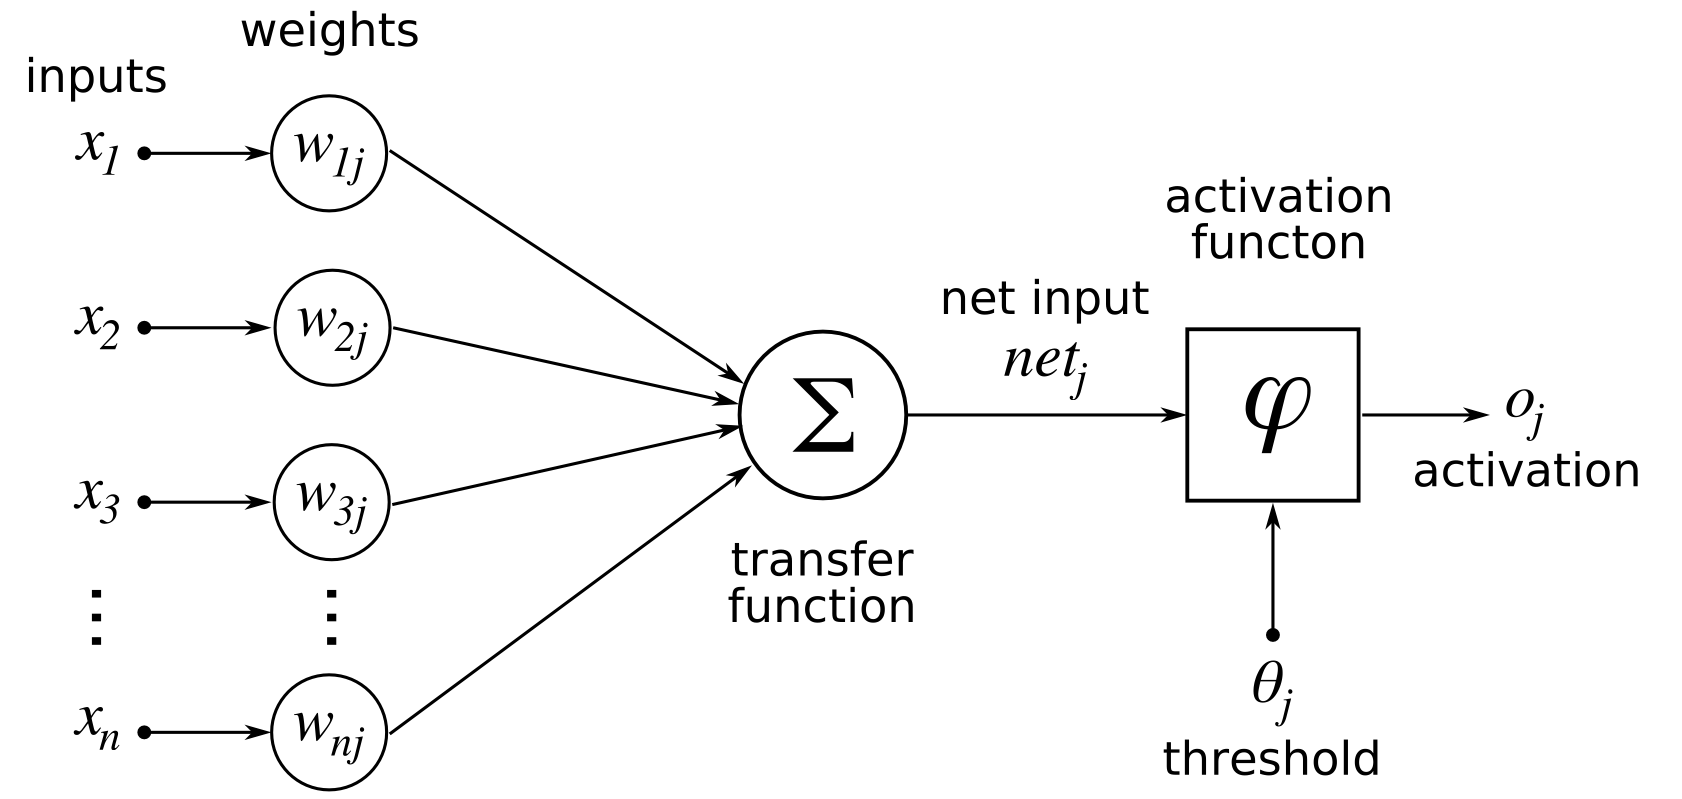
\includegraphics[width=.7\textwidth]{images/ArtificialNeuronModel}} 
	\caption{Artificial Neuron Model}
	\label{fig:Modello matematico di un neurone artificiale}
\end{figure}

\subsection{Funzioni di attivazione}
\label{subsec:fattivazione}
Una funzione di attivazione è una componente fondamentale del modello. Essa consente alla rete di imparare trasformazioni non lineari, in modo da essere in grado di calcolare problemi non banali utilizzando un limitato numero di nodi.

Una delle funzioni più utilizzate è la \emph{sigmoide} $\sigma(x)$, la quale modella la frequenza degli stimoli emessi, da neurone inattivo, $\sigma(x)=0$, a neurone completamente saturo con una frequenza di attivazione massima, $\sigma(x)=1$.

\begin{equation}
\sigma(x) = \frac{1}{1+e^{-x}}
\label{eq:sigmoid}
\end{equation}


Negli ultimi anni è diventata molto popolare la \emph{Rectified Linear Unit} (ReLU) \cite{nair2010rectified,hahnloser2000digital,hahnloser2003permitted,glorot2011deep}, definita dalla seguente equazione:
\begin{equation}
f (x) = \max(0, x)= \begin{cases}
x \quad \mbox{se } x>0\\
0 \quad \mbox{altrimenti}
\end{cases}
\label{eq:relu}
\end{equation}
Questa funzione azzera tutti i valori negativi, mentre ritorna invariati quelli positivi.

Essa viene utilizzata per la sua capacità di accelerare notevolmente il processo di ottimizzazione, inoltre la sua implementazione risulta semplice ed efficiente.

\begin{figure}[htb]
	\centering
	\subfloat[][\emph{Sigmoide}]
	{\includegraphics[width=.45\textwidth]{images/signmoid2}}
	\quad
	\subfloat[][\emph{ReLU}]
	{\includegraphics[width=.45\textwidth]{images/relu2}} 
	
	\caption{Andamento di due funzioni di attivazione}
	\label{fig:subfig}
\end{figure}

\section{Architetture}
\label{sec:architetture}

I neuroni vengono organizzati in una struttura detta architettura della rete.
I dati, partendo da un livello iniziale, chiamato layer di input, attraversano i multipli strati interni della rete, gli hidden layer, raggiungendo l'ultimo livello detto layer di output.

Quando i collegamenti tra i neuroni formano una struttura senza cicli si parla di reti \emph{feed-forward} \cite{svozil1997introduction}.

\subsection{Layer fully-connected}
\label{subsec:fc}

Un’architettura molto comune nelle reti neurali è una struttura ``densa'', che utilizza \emph{layer fully-connected}, in cui tutti i neuroni del livello precedente sono collegati ad ogni neurone dello strato successivo \cite{sainath2015convolutional}.

Lo scopo di un layer completamente connesso è imparare combinazioni non lineari di feature ad alto livello provenienti dal layer precedente. 
Una struttura di questo tipo è però caratterizzata da un numero di connessioni che cresce molto velocemente, causando un accrescimento del numero di parametri che la rete deve apprendere.
Questo comporta un aumento del costo computazionale e un alto rischio di overfitting, approfondito nella sezione \ref{subsec:overfitting}.

Per questo motivo questi vengono spesso sostituiti dai layer convoluzionali.

\subsection{Layer convoluzionali}
\label{subsec:cnn}
Una rete neurale convoluzionale, in inglese \emph{Convolutional Neural Network} (CNN), è una classe di reti artificiali avanzate e \emph{feed-forward}, composte da uno o più strati convoluzionali seguiti da una serie di livelli completamente connessi \cite{kim2014convolutional}.

Una convoluzione può essere considerata come una funzione a finestra scorrevole, detta \emph{kernel} o filtro, applicata a una matrice. 
Ogni livello applica filtri diversi, in genere centinaia o migliaia, e combina i loro risultati. 
Durante la fase di addestramento, una CNN impara automaticamente i valori dei suoi filtri in base all'attività che si desidera eseguire. 


Due parametri che definiscono il comportamento di un layer convoluzionale sono lo \emph{stride}, che rappresenta il passo di 
convoluzione e viene utilizzato per ridurre le dimensioni spaziali dell'output e il \emph{padding}, che definisce il comportamento dei neuroni lungo 
i bordi dei dati di input. Se viene scelto un padding \emph{valid}, l'output contiene solo i neuroni la cui regione di convoluzione è completamente contenuta nei dati; nel caso di padding \emph{same}, invece, l'output mantiene la stessa dimensione dell'input, utilizzando zero come valore per i dati mancanti.

Le reti convoluzionali sono adatte per elaborare dati visivi e altri dati bidimensionali, ed hanno mostrato ottimi risultati nel riconoscimento di immagini e nella manipolazione del linguaggio naturale \cite{manning1999foundations}.
In quest'ultimo caso, l'input è costituito da frasi o documenti rappresentati come una matrice, in cui ogni riga corrisponde a un token, in genere una parola. Tipicamente, questi vettori sono dei word embeddings (rappresentazioni a bassa dimensione) come word2vec \cite{mikolov2013distributed}, ma potrebbero anche essere vettori unici che indicizzano la parola in un vocabolario. 

Nel \emph{Natural Language Processing} (NLP) utilizziamo filtri che scorrono su righe complete della matrice (parole), pertanto, la loro ``larghezza'' è solitamente uguale alla quella della matrice di input. L'altezza, o la dimensione della regione, può variare, ma le finestre tipicamente scorrono su 2-5 parole per volta. 

Risulta che le CNN applicate ai problemi di NLP funzionino abbastanza bene, un esempio è il modello \emph{bag-of-words} che è stato l'approccio standard per anni e ha portato a risultati piuttosto buoni \cite{wallach2006topic}.

Le CNN sono più facili da addestrare e hanno molti meno parametri da stimare. 
Il minor numero di connessioni e pesi di questa architettura, rende gli strati convoluzionali relativamente economici in termini di memoria e potenza di calcolo necessari.

\subsection{Layer di pooling}
\label{subsec:maxpool}

Il \emph{pooling} è un processo alquanto comune nelle reti neurali, la cui funzione è ridurre progressivamente la dimensionalità spaziale per diminuire la quantità di parametri e la complessità computazionale della rete, mantenendo le informazioni più salienti e controllando anche l'overfitting.

Il layer di pooling opera indipendentemente su ogni slice di profondità dell'input e lo ridimensiona spazialmente, usando l'operazione MAX sul risultato di ogni filtro \cite{karpathy2016cs231n}. 

Una proprietà del pool è che fornisce una matrice di output a dimensione fissa --- in genere richiesta per la classificazione. Ciò consente di utilizzare frasi di dimensioni variabili e filtri di dimensioni variabili, ma ottenere sempre le stesse dimensioni di output da inserire in un classificatore.

\subsection{Batch Normalization}
\label{subsec:normalization}

Durante la fase di addestramento del modello, i parametri di ogni substrato vengono ottimizzati al fine di minimizzare l'errore finale.
Ad ogni iterazione, in ciascuno strato avviene una variazione dell'output, corrispondente ad una variazione nei valori in ingresso al livello successivo.
Questo può rappresentare un problema per la rete, che deve adattare i propri strati ad un continuo cambiamento nell'input. 

Per aumentare la stabilità della rete neurale, velocizzare il training e migliorarne le performance, generalmente viene applicata ad ogni strato una \emph{Batch Normalization}  \cite{ioffe2015batch}, la quale normalizza l'uscita di un precedente livello sottraendo il valore medio di un batch e dividendo il risultato per la sua deviazione standard.
\begin{equation}
	\hat{x}^{(k)}=\frac{x^{(k)}-\mean[x^{(k)}]}{\sqrt{\variance[x^{(k)}]}}
\end{equation}

L'applicazione di questa operazione ad ogni input potrebbe cambiare ciò che il layer può rappresentare. Per questo motivo viene assicurato che la trasformazione inserita nella rete possa rappresentare l'identità, in modo da poter annullare il potenziale effetto della Batch Normalization, nel caso in cui fosse l'azione ottimale.
Dunque viene prevista l'aggiunta di due parametri --- ``deviazione standard'' $\gamma$ e ``media'' $\beta$ --- che la rete impara assieme ai parametri del modello originale, come mostrato nell'equazione \ref{eq:batchnorm}
\begin{equation}
	y^{(k)}=\gamma^{(k)}\hat{x}^{(k)}+\beta^{(k)}\mbox{.}
	\label{eq:batchnorm}
\end{equation}

La \emph{Batch Normalization} può essere utilizzata sia su reti \emph{feed-forward}, sia sulle \emph{reti convoluzionali}.
In questo secondo caso, media e varianza vengono calcolate per ogni filtro.

\section{Apprendimento}
\label{sec:apprendimento}
Per insegnare alla rete a risolvere un determinato problema, occorre una fase di addestramento in cui vengono condotte una serie di osservazioni per stabilire quali valori assegnare ad ogni parametro della rete e trovare un modello ottimale.

Questo processo di apprendimento viene strutturato come un problema di ottimizzazione in cui lo scopo è minimizzare una \emph{funzione di costo}, che misura la distanza tra una soluzione particolare ed una ottima. 

\subsection{Funzione di costo}
\label{subsec:loss}

Una funzione di costo mappa un evento ad un numero reale, il quale ne rappresenta intuitivamente il ``costo''.

Nella strategia adottata si utilizzeranno due diverse funzioni obiettivo: l'\emph{errore quadratico medio} per risolvere il problema di regressione, e la \emph{Softmax Cross Entropy} per il compito di classificazione. Mentre per la costruzione dell'embedding verrà applicata la \emph{Noise Contrastive estimation}.

\subsubsection{Mean Squared Error}
\label{subsubsec:MSE}

Per il task il cui compito è prevedere dei valori reali è comune calcolare lo scostamento tra la quantità prevista dalla rete $(\hat{Y})$ e i valori osservati $Y$ (ground truth). 
 
L'\emph{errore quadratico medio} (MSE) di uno stimatore misura la media dei quadrati degli errori, e viene calcolato come

\begin{equation}
\mse = \frac{1}{n}\sum_{i=1}^{n}(Y_i-\hat{Y}_i)^2 \mbox{.}
\end{equation}

con $n$ numero delle previsioni \cite{wang2009mean}.

\subsubsection{Softmax Cross Entropy}
\label{subsubsec:sce}

Softmax è una funzione di loss comunemente utilizzata per la classificazione. In particolare viene applicata allo strato finale della rete ed addestrata in un regime di entropia incrociata \cite{tang2013deep}.\\
L'entropia incrociata è un indicatore che può essere utilizzato per misurare l'accuratezza delle previsioni. 

Date due variabili casuali discrete $p$ e $q$ definiamo l'entropia nel modo seguente:
\begin{equation}
	H(p,q)=-\sum_{x} p(x) \log q(x)
\end{equation}

in cui $p_{x}$ è la ``vera'' probabilità o distribuzione, mentre $q_{x}$ è la distribuzione ``innaturale'' ottenuta a partire dal modello corrente.

Nella pratica la \emph{Cross Entropy} viene calcolata empiricamente ipotizzando l'equiprobabilità degli eventi, poiché $p$ è ignota. 
Di conseguenza, è ridefinibile come segue

\begin{equation}
H(q)=-\frac{1}{N}\sum_{x} \log q(x)
\end{equation}

dove N è il numero di eventi osservati.

L'obiettivo principale di questa funzione è rendere il risultato della Softmax campionata uguale a quella vera. L'algoritmo si concentra sulla selezione di campioni specifici dalla distribuzione data per ottenere la loss desiderata \cite{liu2016large}.  
L'utilizzo della funzione Softmax ha un effetto considerevole sulle prestazioni. 

\subsubsection{Noise Contrastive estimation}
\label{subsubsec:nce}

La stima contrastiva del rumore è una strategia utilizzata nell'ambito della modellazione linguistica o per la generazione di word embedding dati in input dei corpus molto ampi.

La funzione obiettivo del modello \emph{skip-gram} cerca di trovare rappresentazioni di parole che siano utili per predire le parole circostanti, meglio chiamati contesti, in una frase o in un documento. 
Data una sequenza di parole di addestramento, la funzione obiettivo massimizza la probabilità media di log
\begin{equation}
\frac{1}{T}\sum_{t=1}^{T} \sum_{-c \leq j \leq c, j \neq 0} \log p(w_{t+j} | w_T)
\end{equation}

dove $c$ è la dimensione del contesto di training \cite{mikolov2013distributed}. 

Nell'implementazione del modello \texttt{word2vec}, la formulazione standard dello \emph{skip-gram} definisce la precedente probabilità di log ricorrendo alla funzione Softmax:
\begin{equation}
p_{\theta}(w_{O} | w_{I}) = \frac{\exp({v^{\prime}_{w_{O}}}^{\top} v_{w_{I}})}{\sum_{w=1}^{W} \exp({v^{\prime}_{w}}^{\top} v_{w_I})}
\end{equation}

dove $v_w$ e $v'_w$ sono le rappresentazione vettoriali di input e output e $W$ è il numero delle parole del vocabolario \cite{dyer2014notes}.

In questo modo la previsione di una data parola a partire da un contesto risulta essere un compito computazionalmente intenso, poiché vi sono operazione che coinvolgono l'intero dizionario.

Di conseguenza, un alternativa alla funzione Softmax è l'applicazione della \emph{Noise Contrastive estimation} con campionamento negativo \cite{liu2016classification, viswesvaran2000measurement}. Essa consente un allenamento più veloce e rappresentazioni vettoriali migliori per le parole frequenti.

\subsection{Algoritmi di ottimizzazione}
\label{subsec:optimizer}

Gli algoritmi di ottimizzazione sono necessari per minimizzare il risultato di una determinata funzione obiettivo, la quale dipende dai parametri che il modello deve imparare durante l'addestramento. 

Vengono utilizzate varie strategie e algoritmi di ottimizzazione per aggiornare e calcolare i valori appropriati e ottimali di tale modello, i quali influenzano fortemente l'efficacia del processo di apprendimento.

L'entità dell'aggiornamento è determinata dal tasso di apprendimento $\eta$, in inglese \emph{learning rate}, che garantisce la convergenza al minimo globale, per superfici di errore convesse, e ad un minimo locale, per superfici non convesse. 

\subsubsection{Stochastic Gradient Descent}
\label{subsubsec:SGD}

La discesa del gradiente, in inglese \emph{Gradient Descent} (GD), è un algoritmo iterativo per l'ottimizzazione di funzioni \cite{ruder2016overview}.

Viene utilizzato principalmente per eseguire gli aggiornamenti dei pesi in un modello di rete neurale nel seguente modo
\begin{equation}
\theta = \theta - \eta \nabla J(\theta)
\end{equation}
dove $\eta$ rappresenta il tasso di apprendimento, $\nabla J(\theta)$ è il gradiente della funzione di loss $J(\theta)$ rispetto al parametro $\theta$. 

La tradizionale discesa gradiente, o \emph{Batch Gradient Descent} (GD), calcola il gradiente dell'intero set di dati, eseguendo un solo aggiornamento. Di conseguenza il processo di addestramento può risultare lento e difficile da controllare per i set di dati che sono molto grandi. 

I problemi che si verificano con questo algoritmo vengono risolti applicando una sua variante: la {discesa stocastica del gradiente}, in inglese \emph{Stochastic Gradient Descent} (SGD).
Questa tecnica esegue un aggiornamento alla volta dei parametri per ognuno degli esempi di training
\begin{equation}
\theta = \theta - \eta \nabla J(\theta; x(i); y(i))
\end{equation}

dove $x(i)$ e $y(i)$ sono le coppie di esempi usati per l'addestramento.

Questa tecnica risulta essere molto più veloce di quella classica. 
A causa dei frequenti aggiornamenti, i parametri presentano un'alta varianza, inoltre la funzione loss oscilla tra diverse intensità. Questo favorisce la scoperta di nuovi minimi locali, complicando però la convergenza all'ottimo globale. 


\subsubsection{Adagrad}
\label{subsubsec:adagrad}

\emph{Adagrad} è un metodo di apprendimento adattativo che aggiusta il learning rate sulla base dei parametri \cite{duchi2011adaptive} .
In questo algoritmo, la dimensione degli aggiornamenti è grande per parametri associati a caratteristiche poco ricorrenti e piccola per quelli più frequenti. Per questo motivo viene considerato adatto alla gestione di dati sparsi.

Adagrad modifica il tasso di apprendimento generale $\eta$ ad ogni istante di tempo $t$ per ogni parametro $\theta(i)$, sulla base dei gradienti che sono stati calcolati per $\theta(i)$.

Il vantaggio principale di questo metodo è che non è necessario regolare manualmente la frequenza di apprendimento e nella maggior parte delle implementazioni viene usato un valore predefinito --- per esempio \numprint{0,001} --- e lasciato invariato.\\
La principale debolezza consiste nell'accumulo dei ``gradienti quadrati'' nel denominatore, finché ogni termine aggiunto è positivo \cite{ruder2016overview}. Di conseguenza il tasso di apprendimento si riduce fino al punto in cui l'algoritmo non è più in grado di acquisire ulteriori conoscenze. 

\subsection{Paradigmi di apprendimento}
\label{subsec:Paradigmi di apprendimento}

Gli algoritmi di apprendimento sono principalmente suddivisi in due categorie:
\begin{itemize}
	\item[\bfseries supervisionato] --- alla rete viene presentato un training set preparato da un ``insegnante esterno'', composto da coppie significative di valori (input, output atteso).
	
	Quando alla rete neurale viene fornito l'input dall'ambiente, l'insegnante calcola l'output desiderato corrispondente, addestrando la rete mediante un algoritmo (tipicamente quello di back propagation \cite{horikawa1992fuzzy}). 
	
	La rete impara a riconoscere la relazione incognita che lega le variabili di ingresso e uscita, in modo da prevedere il valore di output per qualsiasi valore di ingresso, basandosi solo su una casistica di corrispondenze (coppie input-output).
	
	\item[\bfseries non supervisionato] --- alla rete vengono presentati solo i valori di input, mentre non sono messe a disposizione le informazioni di ritorno dell'ambiente sui valori obiettivo che si vogliono ottenere in risposta o riguardo la correttezza dell'output fornito.
	
	La rete è in grado di individuare da sola pattern, caratteristiche, similarità e regolarità statistiche nei dati di input, acquisendo la capacità di dividerli in cluster rappresentativi che sviluppino delle rappresentazioni interne, senza usare confronti con output noti.
	
	In questo caso, gli algoritmi che modificano i pesi della rete fanno riferimento solo ai dati contenuti nelle variabili di ingresso.
	
	Questo è un tipo di apprendimento autonomo senza controllo esterno sull'errore. È un approccio adatto per ottimizzare le risorse nel caso in cui non si conoscano a priori i gruppi in cui dividere l'input.
\end{itemize}

\section{Train, Validation e Test Sets}
\label{sec:set}
Per misurare le prestazioni di una rete neurale dopo la fase di apprendimento, viene creato un test set formato da coppie non utilizzate per il training e validation set.\\
Vengono generalmente definiti: 
\begin{itemize}
	\item Training set --- sul quale viene eseguito l'algoritmo di apprendimento.
	\item Validation set --- viene utilizzato per regolare i parametri, selezionare le features e prendere decisioni per quanto riguarda l'algoritmo di apprendimento.
	\item Test set --- si utilizza per valutare le performance dell'algoritmo, ma non per prendere decisioni su quale algoritmo di apprendimento o parametri utilizzare. 
\end{itemize}

Una volta definiti i set, ci si concentrerà sul miglioramento delle prestazioni del training e validation set. 

Generalmente la dimensione del test set è un terzo di quella del training. Esso è composto da input critici su cui la risposta della rete deve essere buona. 
Questo funziona bene quando sono messi a disposizione un numero limitato di esempi, ma nell'era dei Big Data, dove i problemi di apprendimento automatico consistono di più di un miliardo di campioni, la frazione di dati allocati agli insiemi di sviluppo e test è ridotta, nonostante il valore assoluto di esempi sia maggiore.

Vengono utilizzate diverse tecniche statistiche per valutare la bontà di un modello.

\subsection{Evaluation metric}
\label{subsec:EvaluationMetric}

Le metriche di valutazione misurano le prestazioni di un modello, discriminando la bontà dei risultati ottenuti.
Vengono presi in considerazione diversi tipi di metriche per valutare i modelli. La scelta della metrica dipende completamente dal tipo di modello e dal piano di implementazione. 

I modelli predittivi si distinguo in due principali categorie: si parla di \emph{regressione} quando l'output da prevedere è continuo, o di \emph{classificazione} nel caso in cui l'output sia nominale o binario. 
\subsubsection{Regressione}
\label{subsubsec:regressione}

L'{scarto quadratico medio}, in inglese \emph{Root Mean Squared Error} (RMSE), è la metrica di valutazione più popolare utilizzata nei problemi di regressione. Questo parametro aiuta a fornire risultati affidabili, mostrando correttamente la grandezza del termine di errore.
La metrica RMSE è definita dalla seguente equazione
\begin{equation}
	\rmse = \sqrt{\frac{\sum_{i=1}^{N}({Y}_i - \hat{Y}_i)^2}{N}} \mbox{.}
	\label{eq:rmse}
\end{equation}

con $\hat{Y}$ quantità prevista dalla rete, $Y$ i valori osservati e $N$ numero delle previsioni.
\subsubsection{Classificazione}
\label{subsubsec:classificazione}

Nei problemi di classificazione, in particolare quella binaria, gli output sono 0 o 1. \\
Una \emph{matrice di confusione}, nota anche come matrice di errore, è una tabella $2 \times 2$, generalizzabile ad una $N \times N$ per problemi ad $N$ classi, che consente la visualizzazione delle prestazioni di un algoritmo di apprendimento supervisionato. 

Ogni colonna della matrice rappresenta le istanze previste di una classe mentre ciascuna riga quelle osservate. 

\begin{figure}[t]
	\centering
	{\includegraphics[width=.3\textwidth]{images/confmatrix}}
	\caption{Visualizzazione di una matrice di confusione}
	\label{fig:confmat}
\end{figure}

L'individuazione di falsi positivi (casi negativi identificati come positivi), falsi negativi (casi positivi identificati come negativi), veri positivi (casi positivi correttamente identificati) e veri negativi (casi negativi correttamente identificati), mostrati nella figura \ref{fig:confmat}, consentono  un'analisi più dettagliata della semplice proporzione di classificazioni corrette.

È possibile estrarre da questa tabella le seguenti misure di performance:
\begin{itemize}
	\item l'\emph{accuracy}, o accuratezza, del modello, che consiste nella porzione rispetto al totale delle previsioni corrette
	\begin{equation}
		\frac{\mbox{True Positive} + \mbox{True Negative}}{\mbox{True Positive} + \mbox{True Negative} + \mbox{False Positive} + \mbox{False Negative}}
	\end{equation} 
	\item la \emph{precision}, o precisione, cioè la porzione dei casi positivi identificati correttamente
		\begin{equation}
	\frac{\mbox{True Positive}}{\mbox{True Positive} + \mbox{False Positive}}
	\end{equation}
	
	\item la \emph{recall}, ovvero la porzione dei casi positivi reali correttamente identificati
		\begin{equation}
	\frac{\mbox{True Positive}}{\mbox{True Positive} + \mbox{False Negative}}
	\end{equation}
\end{itemize}


\subsection{Overfitting}
\label{subsec:overfitting}

L'\emph{overfitting} è ``la produzione di un'analisi che corrisponde esattamente a un particolare insieme di dati o ne presenta forti similarità; può determinare l'impossibilità di adattamento a nuovi dati o compromettere l'affidabilità delle predizioni sulle osservazioni future''.

La rete neurale deve avere la capacità di comprensione del modello statistico dei dati. In presenza di overfitting essa memorizza i dati del training set e non è quindi in grado di generalizzare su nuovi dati. L'essenza di questo problema consiste nell'estrarre inconsapevolmente parte della variazione residua (cioè il rumore) come se quella variazione rappresentasse la sottostante struttura del modello \cite{burnham2003model}.

Per ridurre la possibilità di overfitting esistono diverse tecniche, come la convalida incrociata (Cross Validation), la regolarizzazione o l'\emph{early stopping}, che consiste nell'utilizzo di un validation set di coppie non usate nel training set per la misurazione dell'errore.

\chapter{Formulazione}
\label{chap:formulazione}

\section{Definizione del problema }
\label{sec:problem}

Partendo da materiale testuale presente in rete, in particolare un dataset messo a disposizione da \emph{Yelp Dataset Challenge} contenente \numprint{5200000} reviews relative a \numprint{174000} business di 11 aree metropolitane nel mondo, l'obiettivo è quello di estrarre da questi dati caratteristiche di personalità.\\ 
Il nostro scopo è di identificare un adeguato spazio semantico che permetta di definire la personalità dell'oggetto target a cui un determinato testo si riferisce.

\section{Descrizione del dataset}
\label{sec:dataset}

Come punto di partenza, viene messo a disposizione un dizionario di 637 aggettivi, che la letteratura psicologica definisce come marker dei cinque grandi tratti di personalità noti come \emph{Big Five}.
In particolare, questo vocabolario associa ad ogni aggettivo un vettore di cinque elementi in cui ogni elemento corrisponde al grado di presenza o assenza di una determinata caratteristica.
\begin{figure}[H]
	\centering
\begin{tabular}{lccccc}
	\toprule
	 \textbf{Adjective} \quad & \multicolumn{5}{c}{\textbf{OCEAN}} \\
	
\midrule
	Active  & 0,053194 & 0,237406 & 0,365915 & 0,116700 & -0,058669  \\
	Angry  & -0,004604 & -0,038453 & 0,020755 & -0,294754 & 0,590114 \\
	Boring & -0,069877 & -0,099754 & -0,478821 & -0,236462 & 0,118821\\
	\rule{7pt}{0\normalbaselineskip} \dots &   \dots 		&			 \dots &			\dots &			 \dots & \dots \\
	\bottomrule
\end{tabular}
\captionof{table}{Esempio di dizionario OCEAN}
\label{tab:ocean}
\end{figure}

\section{Calcolo della Ground Truth}
\label{sec:GroundTruth}

Per poter addestrare correttamente il modello è necessario avere una Ground Truth, ovvero una label associata ad ogni input della rete. Senza questa informazione sarebbe impossibile ottimizzare il modello e valutarne la validità. 

Si procede eliminando dal dataset tutte le sentences non contenenti almeno uno degli aggettivi presenti nel dizionario OCEAN. In seguito verranno utilizzati i dati contenuti all'interno del vocabolario per creare una mappatura diretta tra ogni frase e il corrispondente vettore di personalità, in cui ogni elemento sarà calcolato come la media del valore di ogni aggettivo presente nel testo.

\section{Preprocessing}
\label{sec:preprocessing}
Gli algoritmi di apprendimento automatico non sono in grado funzionare direttamente con il testo non elaborato, è quindi necessario eseguire in primis un preprocessamento del nostro database di testi e in seguito convertire i nostri dati in numeri, nello specifico, in vettori di numeri.\\
Alla fine di questo processo il dataset ottenuto sarà suddiviso in tre corpora: 
\begin{itemize}
	\item \SI{70}{\percent} training set : contenente \numprint{4351900} reviews utilizzate dalla rete per l'apprendimento;
	\item \SI{10}{\percent} validation set: contenente \numprint{621700} reviews;
	\item \SI{20}{\percent} testing set: contenente \numprint{1243000} reviews.
\end{itemize}
La divisione dei tre dataset dovrà mantenere una buona distribuzione fra le diverse classi.

\subsection{Natural Language Processing}
\label{subsec:nlp}
Il \emph{Natural Language Processing} (NLP) è un insieme di tecniche di computer science e linguistica che ricorrono a dei calcolatori per analizzare il linguaggio umano.
\\

Dal punto di vista sintattico ecco una serie di operazioni che vengono applicate al dataset:
\begin{itemize}
	\item \textbf{Rottura della frase}: dato un pezzo di testo vengono trovati i limiti della frase, spesso contrassegnati da punti o altri segni di punteggiatura.
	\item \textbf{Stemming}: alcune parole vengono ridotte alla loro forma radice (ad esempio ``argue, argued, argues, arguing, and argus'' sono mappati alla parola ``argu'').
	\item \textbf{Segmentazione di parole}: un blocco di testo o sentence viene separato in parole. Per una lingua come l'inglese, questo è abbastanza banale, poiché le parole sono solitamente separate da spazi. 
	{\color{orange}	\item \textbf{Estrazione terminologica}: L'obiettivo dell'estrazione terminologica è estrarre automaticamente i termini rilevanti da un dato corpus.}
\end{itemize}
Dal punto di vista semantico invece si interviene nel seguente modo:
\begin{itemize}
	\item \textbf{Semantica lessicale}: tenta di comprendere il significato computazionale delle singole parole nel loro contesto.
	\item \textbf{Comprensione del linguaggio naturale}: i blocchi di testo vengono convertiti in rappresentazioni più formali più facili da manipolare per i programmi di computer. 
	\item \textbf{Segmentazione e riconoscimento degli argomenti}: data una porzione di testo, separarla in segmenti ciascuno dei quali è dedicato a un argomento e identifica l'argomento del segmento.
\end{itemize}
Ricorrendo, dove possibile, alle tecniche sopraelencate, è possibile costruire un dizionario delle \numprint{60000} parole più frequenti nel corpus di training, basato sulla frequenza assoluta di una parola, avendo cura di eliminare tutti gli aggettivi presenti nel dataset OCEAN.

\begin{figure}[H]
	\centering
	{\includegraphics[width=.8\textwidth]{images/dict_histogram30}}
	\caption{Istogramma rappresentativo delle \num{30} parole più frequenti nel dizionario}
	\label{fig:Istrogramma del dizionario}
\end{figure}
In questo modo non verrà influenzata la rete mostrando l'associazione tra gli aggettivi e le label associate, ed il modello sarà ``costretto'' ad imparare il legame esistente tra il contesto di una frase e il relativo valore del tratto di personalità. 

Inoltre sarà necessario anche rimuovere tutte le \emph{stopwords} relative alla lingua inglese, ovvero parole considerate poco significative perché usate troppo frequentemente all'interno delle frasi --- per esempio gli articoli e le congiunzioni --- filtrando i termini comuni e senza uno specifico significato semantico dalle parole che trasportano vere informazioni.

In seguito ogni parola del dizionario verrà codificata con un valore intero univoco, mentre quelle non presenti, tra cui gli aggettivi mappati nel vocabolario OCEAN, verranno indicizzati al valore ``-1'' e gli verrà associato il token 'UNK' come mostrato nella figura \ref{fig:preprocessing}
\begin{figure}[H]
	\centering
	{\includegraphics[width=.5\textwidth]{images/preprocessing}}
	\caption{Visualizzazione del preprocessing}
	\label{fig:preprocessing}
\end{figure}


\chapter{Esperimenti e risultati}
\label{chap:esperimenti}

I precedenti modelli di previsione della personalità si sono concentrati sull'applicazione di tecniche generali di apprendimento automatico per predire i tratti di personalità Big Five.
In particolare verranno utilizzate diverse strutture di rete, combinando differenti domini.

\section{Spazi di rappresentazione}
\label{sec:approcci}
Per affrontare questo problema di \emph{Text Mining}, gli esperimenti si concentrano su due principali metodi per l'estrazione delle caratteristiche:
\begin{itemize}
	\item Un approccio supervisionato, in cui viene utilizzato come strumento di generazione di feature un vettore \emph{bag-of-words} o brevemente BoW, una rappresentazione di testo che descrive la presenza delle parole all'interno di un documento, in questo caso nel dizionario delle occorrenze.
	\item Un approccio non supervisionato, in cui viene costruito un embedding, tramite gli algoritmi di Mikolov. Insegnando alla rete il significato delle parole e la relazione tra di esse, è possibile rappresentare, sotto forma di vettori, le mappature tra le parole e i contesti.
\end{itemize}
$\\$
In seguito viene posta l'attenzione su tre diverse architetture neurali:
\begin{itemize}
	\item Reti fully-connected;
	\item Reti neurali convoluzionali CNN;
	\item Classificatori multi-label binari.
\end{itemize}



\section{Esperimento 1}
\label{sec:es1}
\subsection{Input Features}
\label{subsec:features1}

Nel primo approccio proposto, per rappresentare i dati testuali viene utilizzato il modello \emph{bag-of-words}, un tipo di descrizione semplificata, spesso utilizzata nell'elaborazione del linguaggio naturale e nel campo dell'\emph{Information Retrivial} (IR). 

Sfruttando il dizionario delle occorrenze precedentemente costruito, il testo viene modellato  come fosse una ``borsa di parole'', in cui grammatica e ordine delle parole vengono trascurate.
Ogni frase viene ridotta ad un vettore in cui ogni elemento identifica una parola del dizionario. Nella posizione corrispondente ad un determinato termine vi sarà il valore \num{1} se la parola è contenuta nella frase, \num{0} altrimenti.

Il modello riguarda solo le parole conosciute, di conseguenza i vocaboli che compaiono nel testo ma sono assenti nel dizionario vengono trascurati.

\begin{figure}[H]
	\centering
	{\includegraphics[width=.6\textwidth]{images/bow}}
	\caption{Visualizzazione del modello \emph{bag-of-words}}
	\label{fig:bow}
\end{figure}

\subsection{Architettura della rete}
\label{subsec:modelli1}

Una volta estratte, le features posso essere passate in input alla rete neurale, che le elabora calcolando le risposte dei neuroni dal livello di input verso il livello di output.

In questa prima strategia viene utilizzata una rete \emph{feedforward}, in cui le informazioni si spostano dal livello di input attraverso eventuali strati nascosti fino al livello di output senza cicli. L'architettura è caratterizzata da una struttura densa o \emph{fully-connected}, in cui tutti i neuroni del layer precedente sono collegati ad ogni neurone del layer successivo, e ciascuna connessione ha il proprio peso.


Lo scopo di un layer completamente connesso è imparare combinazioni non lineari di feature ad alto livello provenienti dal layer precedente. L'ultimo di questi strati rappresenta l’output della rete.

Ad ogni livello fully connected viene applicata la funzione di attivazione non lineare \emph{ReLU}, descritta nella sezione \ref{subsec:fattivazione}.

Inoltre, per accelerare l'apprendimento ed aumentare la stabilità della rete, effettuiamo dopo ogni layer una \emph{batch normalization}, definita nella sezione \ref{subsec:normalization}. {\color{red}in realtà non mi pare si sia descritto come funziona in quella sezione, decida come desidera trattare questi aspetti per evitare che le vengano mosse obiezioni}

Vengono presentate nella tabella \ref{tab:arcbow+fc} tre architetture implementate, con differenti strati e numero di neuroni che caratterizza ciascuno.


\begin{figure}[H]
	\centering
		\begin{tabular}{lcccc}
			\toprule
			\textbf{Layer} \quad & \textbf{Modello 1} & \textbf{Modello 2} & \textbf{Modello 3} &  \textbf{Modello 4}  \\
			\midrule
			Input 				 & \numprint{60000}	  & \numprint{60000}   &\numprint{60000}	&\numprint{60000}	   \\
			fc1  				 & \num{300}		  & \num{300} 		   & \num{100} 			& \num{300} 		   \\
			fc2  				 &  \num{200}		  & \num{200} 		   & \num{50}  			& \num{20}  		   \\
			fc3					 & -				  & \num{100} 		   & \num{20} 			& -					   \\
			Output 				 &  \num{5}			  & \num{5} 		   & \num{5}			& \num{5} 			   \\
			\bottomrule
		\end{tabular}
	\captionof{table}{Confronto delle architetture di tre differenti modelli}
	\label{tab:arcbow+fc}
\end{figure}

Tutte le simulazioni sono state addestrate per \num{10} epoche: la fase di addestramento viene in genere portata avanti fino a quando le performance sul test non producono alcun miglioramento.

L’ottimizzatore scelto è l'{Adaptive Subgradient Methods} \emph{Adagrad}, introdotto nella sezione \ref{subsubsec:adagrad}, con learning rate \numprint{0,001}.

Come funzione di loss è stato scelto l'errore quadratico medio, in inglese \emph{mean squared error (MSE)}, presentato nella sezione \ref{subsec:loss}. Mentre la metrica di valutazione utilizzata per misurare le prestazioni predittive del modello è la \emph{root mean squared error} (RMSE), introdotta nella sezione \ref{subsec:EvaluationMetric}.

In ogni epoca si alternano una fase di training ed una fase di test in modo tale da monitorare costantemente i miglioramenti o i peggioramenti del modello sul test set. 

\subsection{Performance}
\label{subsec:performance1}
Prendendo in considerazione le tre diverse architetture implementate, presentiamo i nostri risultati ottenuti in termini di loss.
\begin{table}[H]
	\centering
	\begin{tabular}{l@{\hspace{.5cm}}ccc}
		\toprule
		 & \textbf{Dev loss} & \textbf{Test loss} & \textbf{Tempo di training}  \\
		\midrule
		\textbf{Modello 1} & \numprint{0.0607} & \numprint{0.0619} &\numprint{235} min \\
		\textbf{Modello 2} & \numprint{0.0901} & \numprint{0.0606} &\numprint{250} min \\
		\textbf{Modello 3} & \numprint{0.0680} & \numprint{0.0624} &\numprint{265} min \\
%		\textbf{Modello 4} & \numprint{0.0287} & \numprint{0.0104} &\numprint{145} min \\
		\bottomrule 
	\end{tabular}
	\captionof{table}{Confronto dei risultati in termini di \emph{loss} ottenuti dalle tre diverse reti}
	\label{tab:lossbow+fc}
\end{table}

Per valutare l'efficacia di questi modelli, è fondamentale eseguire un analisi dettagliata, in particolare ponendo l'attenzione sui valori di RMSE per ogni tratto di personalità.
Calcolando il valore medio assunto da ogni caratteristica durante la fase di addestramento, è possibile stabilire qual è il valore di root mean squared error di un modello concettuale che per ogni tratto predice sempre il suo valore medio.
 
\begin{table}[H]
	\centering
	\begin{tabular}{clccccc}
		\toprule	
		& 		  & \multicolumn{5}{c}{\textbf{Root Mean Squared Error}} 									    \\
		\multicolumn{2}{c}{\multirow{-2}{*}{Modelli}}
		& O 				& C 			   & E 				  & A 				 & N 			    \\ 
		\midrule
		\multirow{2}*{\textbf{Modello 1}} & Modello   & \numprint{0,148} & \numprint{0,227} & \numprint{0,224} & \numprint{0,251} & \numprint{0,351} \\
		& Modello 0 & \numprint{0,145} & \numprint{0,224} & \numprint{0,213} & \numprint{0,218} & \numprint{0,318} \\
		\midrule
		\multirow{2}*{\textbf{Modello 2}} & Modello   & \numprint{0,147} & \numprint{0,226} & \numprint{0,225} & \numprint{0,251} & \numprint{0,341} \\
		& Modello 0 & \numprint{0,141} & \numprint{0,227} & \numprint{0,213} & \numprint{0,208} & \numprint{0,305} \\
		\midrule
		\multirow{2}*{\textbf{Modello 3}} & Modello   & \numprint{0,147} & \numprint{0,226} & \numprint{0,225} & \numprint{0,262} & \numprint{0,348} \\
		& Modello 0 & \numprint{0,233} & \numprint{0,307} & \numprint{0,262} & \numprint{0,373} & \numprint{0,546}  \\
%		\midrule
%		\multirow{2}*{\textbf{Modello 4}} & Modello   & \numprint{0,147} & \numprint{0,226} & \numprint{0,225} & \numprint{0,262} & \numprint{0,348} \\
%		& Modello 0 & \numprint{0,233} & \numprint{0,307} & \numprint{0,262} & \numprint{0,373} & \numprint{0,546}  \\
		\bottomrule	
	\end{tabular}
	\captionof{table}{Confronto dei risultati in termini di \emph{Root Mean Squared Error} delle architetture contro il modello basato sulla media di training}
	\label{tab:confmm0bow+fc}
\end{table}

{\color{red} sembrerebbe leggermente meglio il terzo modello}
Mettendo a confronto le due metriche, si nota che i modelli realmente implementati imparano nella maggioranza dei casi a predire un valore con lo stesso errore commesso dai modelli banali che calcolano la media. Risulta allora evidente che i risultati ottenuti non siano ottimali.

La scarsa efficienza di questi modelli potrebbe dipendere dall'efficacia con cui vengono codificate le feature in input alla rete. 
Infatti le limitazioni dell'approccio bag-of-words derivano in parte dalla progettazione del vocabolario e della sua dimensione, che può causare una scarsa ``descrizione'' del documento. 
Scartare l'ordine delle parole e ignorare il contesto non consente di determinare la differenza tra le stesse parole disposte diversamente, i sinonimi ecc.
Inoltre, un tipo di rappresentazione sparsa risulta più difficile da modellare quando si cercano modelli in grado di sfruttare poche informazioni in uno spazio rappresentativo ampio, sia per ragioni computazionali (spazio e complessità temporale) sia per ragioni di informazione.

\section{Esperimento 2}
\label{sec:es2}

In compiti come il riconoscimento di parole, tutte le informazioni ed ogni termine vengono rappresentati per mezzo di id unici e discreti.
Queste codifiche però non forniscono alcuna informazione utile al sistema riguardo le relazioni che possono sussistere tra i singoli elementi. Ciò significa che il modello può sfruttare molto poco di ciò che ha appreso su una determinata parola quando sta elaborando i dati. 

Questo tipo di ``raffigurazione'' porta alla creazione di dati sparsi, di conseguenza, per ottenere un modello di successo, potrebbero essere necessari più dati di input. 

L'utilizzo di modelli spaziali vettoriali (VSM) per rappresentare le parole in uno spazio continuo, può aiutare a superare alcuni dei sopracitati ostacoli.
Questi metodi dipendono dall'ipotesi distributiva, la quale afferma che le parole che appaiono negli stessi contesti condividono lo stesso significato semantico \cite{FIXME}. 

\subsection{Input Features}
\label{subsec:features2}

Nel secondo approccio, viene utilizzato un modello spazio-vettoriale, in particolare viene adottata una tecnica non supervisionata, che consiste nell'implementazione e applicazione del modello \texttt{word2vec} di Tomas Mikolov \cite{mikolov2013efficient}. 

\texttt{Word2vec} è un modello predittivo particolarmente efficiente dal punto di vista computazionale per l'apprendimento degli embedding di parole dal testo non elaborato. 
Esso consiste in una rete neurale a due strati, addestrati a ricostruire i contesti linguistici delle parole. 
\\
\\
L'algoritmo prende in input un grande corpus di testo, producendo uno spazio vettoriale, in genere di diverse centinaia di dimensioni. Ogni parola univoca nel corpo che viene assegnata a un vettore corrispondente nello spazio. 

Per l'implementazione viene utilizzato il modello \emph{Skip-Gram}, una versione di questo algoritmo che predice le parole di contesto di origine a partire dalle parole target \cite{FIXME}.

A partire dal dataset, viene formato un set che accoppia ogni parola target ai contesti in cui appare. Viene considerato come contesto l'insieme delle ``parole a sinistra'' e delle ``parole alla destra'' dell'obiettivo, ovvero la finestra di parole, di dimensione 1, attorno al target. 
In questo modo, ogni coppia di destinazione del contesto viene trattata come se fosse una nuova osservazione, incrementando le informazioni distribuzionali.\\

\begin{figure}[htb]
	\centering
	{\includegraphics[width=.75\textwidth]{images/skip-gram}} 
	\caption{Visualizzazione del modello Skip-gram}
	\label{fig:mikolov}
\end{figure}

In questo tipo di apprendimento, i vettori si posizionano nello spazio in modo tale che le parole che condividono contesti comuni nel corpo siano situate in stretta prossimità l'una dell'altra, in altri termini, vocaboli semanticamente simili sono mappati a punti vicini dello spazio.\\
Un esempio interessante viene illustrato nella figura \ref{fig:embedding1}\subref{subfig:vis3d} --- si ponga particolare attenzione alle parole ``beautiful'', ``lovely'', ``chic'', ``trendy'' ecc..

\begin{figure}[htb]
	\centering
	\subfloat[][\emph{Visualizzazione 2D}\label{subfig:vis2d}]
	{\includegraphics[width=.45\textwidth]{images/embedding1/embedding1_tsne_2d}}
	\hspace{10mm}
	\subfloat[][\emph{Dettaglio di una visualizzazione 3D}\label{subfig:vis3d}]
	{\includegraphics[width=.45\textwidth]{images/embedding1/Embedding1_similarity}}
	
	\caption{Proiezione dell'embedding di Mikolov nello spazio 2-3 dimensionale, tramite la \emph{tecnica di riduzione della dimensionalità} (t-SNE) \cite{FIXME}.}
	\label{fig:embedding1}
\end{figure}

%La funzione obiettivo viene definita sull'intero set di dati, ma ottimizzata con la discesa del gradiente stocastico (SGD) un esempio alla volta 

\subsection{Architettura della rete}
\label{subsec:modelli2}


%Windowing, parole attorno agli aggettivi della lista degli aggettivi disponibili:
%K parole prima e dopo la parola corrente, finestre scorrevoli





\subsection{Performance}
\label{subsec:performance2}



%\subsection{Layer convoluzionale}
%\label{subsec:layerconv}
%Livello denso / completamente connesso: un'operazione lineare sul vettore di input del livello.
%Livello involutivo: un livello costituito da un insieme di "filtri". I filtri accettano un sottoinsieme dei dati di input alla volta, ma vengono applicati all'intero input (passando sopra l'input). Le operazioni eseguite da questo livello sono ancora moltiplicazioni lineare / matrice, ma passano attraverso una funzione di attivazione all'uscita, che di solito è un'operazione non lineare.
%Pooling layer: utilizziamo il fatto che livelli consecutivi della rete sono attivati da caratteristiche "più alte" o più complesse che sono esposte da una vasta area dei dati di input della rete. Un livello di raggruppamento riduce in modo efficace i campioni dell'output del livello precedente, riducendo il numero di operazioni richieste per tutti i livelli successivi, ma passando comunque le informazioni valide dal livello precedente.
%Livello di normalizzazione: utilizzato per l'input per il ridimensionamento delle funzionalità e per la normalizzazione batch nei livelli nascosti.
%
%
%
%Uno strato convoluzionale è molto più specializzato ed efficiente di uno strato completamente connesso.
%
%
%
%Al contrario, in uno strato convoluzionale ogni neurone è collegato solo a pochi neuroni vicini (alias locali) nel livello precedente, e lo stesso insieme di pesi (e layout di connessione locale) è usato per ogni neurone.
%
%Il minor numero di connessioni e pesi rende gli strati convoluzionali relativamente economici (rispetto alla piena connessione) in termini di memoria e potenza di calcolo necessari.
%Il nome strato / rete "convoluzionale" deriva dal fatto che il modello di connessione locale e lo schema di peso condiviso possono essere interpretati come un filtro (o un insieme di filtri) che viene "convogliato" con l'input / immagine ... Ma in inglese semplice è solo un "layer di peso condiviso localmente connesso".
%
%Embedding
%Deep representation
%Fully connected part
%
%
%EMBEDDING
%Incorporando i livelli prendi una sequenza di parole id come input e produci una sequenza di vettori corrispondenti come output. La loro funzionalità è molto semplice e poiché la semantica di questi vettori non è interessante per il nostro problema, l'unica domanda rimanente è "Qual è il modo migliore per inizializzare i pesi?"
%
%A seconda del problema, le risposte possono essere controintuitive come il consiglio "generare le proprie etichette sintetiche, formare word2vec su di esse e avviare il livello di incorporamento con esse".
%
%Ma per tutti gli scopi pratici è possibile utilizzare un set pre-addestrato di incastri e sintonizzarlo congiuntamente per il modello specifico. È probabile che i vettori di parole risultanti cesseranno di dimostrare le stesse proprietà di un modello word2vec vanill:
%
%
%DEEP REPRESENTATION
%Lo scopo principale della parte di rappresentazione profonda è di condensare tutte le informazioni rilevanti nel suo output, mentre sopprime le parti che potrebbero portare a identificare un singolo campione da esso. Ciò è altamente auspicabile in quanto la rete con capacità elevata probabilmente si sovraperforma su particolari esempi e ha prestazioni scarse sul set di test.
%
%Rete neurale convoluzionale (CNN)
%
%Un modo alternativo per addestrare un classificatore di testo profondo consiste nell'utilizzare reti convoluzionali. Tipicamente, dato un campo ricettivo abbastanza grande, è possibile ottenere gli stessi risultati di un livello di attenzione dedicato. Non c'è un singolo trucco qui, ma tenere un sacco di mappe delle caratteristiche all'inizio e ridurre il loro numero in modo esponenziale in un secondo momento aiuta a evitare l'apprendimento di modelli irrilevanti.
%
%
%FULLY CONNECTED PART
%Classificatore denso
%
%Una parte completamente connessa esegue una serie di trasformazioni sulla rappresentazione profonda e alla fine emette i punteggi per ogni classe. La migliore pratica qui è applicare le trasformazioni come segue:
%
%Livello completamente connesso
%Normalizzazione batch
%(Opzionale) Trasformazione non lineare (tangente iperbolica o ELU)
%Buttare fuori
%Spero che vi piaccia questa panoramica degli algoritmi di classificazione del testo neurale che può essere ulteriormente potenziata con metodi più sofisticati di vostra scelta. Alcuni suggerimenti e trucchi menzionati qui ti aiuteranno a costruire modelli migliori e ad ottenere una convergenza più rapida.
%
%Inoltre, qui sotto troverai alcuni link a tutorial e strumenti per compiti di apprendimento di classificazione e rappresentazione.
%
%
%
%Modello di design
%Abbiamo progettato 2 ConvNets, uno grande e uno piccolo. Sono entrambi 9 strati profondi con 6 strati convoluzionali e 3 strati completamente connessi. La figura 1 mostra un'illustrazione
%Lunghezza
%...
%Convoluzioni Conv. Max pooling e piscina. strati completamente connessi
%Figura 1: illustrazione del nostro modello
%L'input ha un numero di caratteristiche pari a 70 a causa del nostro metodo di quantizzazione dei caratteri, e la lunghezza della funzione di input è 1014. Sembra che 1014 caratteri possano già catturare la maggior parte dei testi di interesse. Inseriamo anche 2 moduli di interruzione [10] tra i 3 livelli completamente connessi per la regolarizzazione. Hanno una probabilità di abbandono di 0,5. La Tabella 1 elenca le configurazioni per i layer convoluzionali e la tabella 2 elenca le configurazioni per i layer (lineari) completamente connessi.
%
%
%\section{Struttura}
%\label{sec:struttura}
%Per un tipo di apprendimento supervisionato:\\
%• Individuare le classi in cui dividere l’input secondo il tipo di problema\\
%• Scegliere le feature analizzando matematicamente gli oggetti in input\\
%• Definire molte coppie (input, output) per i set di training (60\%), validation (20\%), test (20\%)\\
%• Definire la codifica numerica: per l’input valori in [-1,1]; per l’output valori binari {0,1}\\
%\\
%Scegliere un modello di rete e definirne l’architettura con:\\
%– Funzione di attivazione per ogni neurone\\
%– Numero di livelli hidden e numero di neuroni per ogni livello hidden (non esistono precise regole per determinarli, solo con tentativi e verifiche degli errori commessi)\\
%– Numero di neuroni per lo strato input: tanti quanti i valori delle feature\\
%– Numero di neuroni per lo strato output: tanti quante sono le classi\\
%• Scegliere un algoritmo di apprendimento e i suoi parametri di controllo (es. back propagation)\\
%• Scegliere una tecnica per controllare l’apprendimento (es. early stopping)\\
%• Scegliere alcuni criteri per valutare la qualità della risposta globale della rete sul test set\\
%\\
%
%
%
%
%
%
%adottiamo diverse tecniche per la costruzione dei modelli.  
%
%tentiamo con diversi esperimenti di identificare ...
%
%Proposti  numerosi  approcci. 
%
%adotteremo
%
%realizzeremo diversi modelli al fine di estrarre informazioni significative...
%
%
%
%
%
%
%
%Vi sono stati numerosi esperimenti prima di ottenere il modello finale, ovvero quello con le performance migliori. Di seguito vengono descritti brevemente soltanto quelli più significativi, mentre per la descrizione precisa del modello finale si rimanda alla sezione successiva.\\
%
%
%
%
%
%L'approccio descritto viene applicato allo stesso modo per ogni coppia di documenti di esperti e corpora di documenti presentati. Costruiamo 6 diversi tipi di modelli 
%
%
%i metodi coinvolti 
%
%sono una tecnica senza supervisione, 
%
%
%Sfruttando i dataset ... generiamo ... per addestrare i modelli ... . 
%
%
%Il primo ... contiene i
%è composto da 
%
%
%il numero di features è 

\section{Risultati}
\label{sec:risultati}

%Abbiamo valutato il nostro approccio basato sulla conoscenza sulla sua efficacia nel predire la personalità degli individui rispetto al modello dei Big Five. La nostra valutazione misura le prestazioni di: 1) classificare gli individui per ogni tratto di personalità e 2) stimare il grado di appartenenza degli individui a ciascun tratto di personalità. La prima valutazione è definita come un problema di classificazione multi-etichetta e assegna etichette "Sì" e "No" per gli individui per ciascun tratto di personalità. Questa è la metodologia di valutazione più popolare seguita nella letteratura sulla previsione della personalità. La seconda valutazione si concentra sul grado di appartenenza di ciascun individuo a ciascun tratto di personalità rispetto all'assegnazione di etichette piuttosto rigide "Sì" e "No". Gran parte della ricerca pertinente in letteratura non ha valutato questa impostazione della previsione della personalità [19]. Riteniamo che questa impostazione sia più vicina allo scenario del mondo reale dal momento che ogni individuo ha alcune caratteristiche da ogni tratto della personalità piuttosto che appartenere a ciascun tratto o meno. La seconda valutazione è definita come un problema di regressione e usiamo la regressione lineare e SVM per la regressione [9] per stimare il valore del grado di appartenenza.
%
%Dataset di valutazione
%Abbiamo utilizzato il famoso repository di dati di Facebook gestito dal progetto "myPersonality" 3 come set di dati di valutazione nei nostri esperimenti. Questo repository viene creato raccogliendo i dati utilizzando la popolare applicazione Facebook "myPersonality" lanciata nel 2007. I valori di personalità degli individui nel set di dati vengono valutati chiedendo loro di fare un test psicometrico standard. L'output di questo test mostra il grado di appartenenza di ciascun individuo a ciascun tratto di personalità e questi valori sono compresi tra 1 e 5. Ad esempio, un individuo può avere valori 2,85 per extraversione, 4,20 per nevroticismo, 2,12 per coscienziosità, 3,55 per gradevolezza e 4.31 per i tratti di personalità di apertura. Attualmente, possiede i dati di milioni di utenti di Facebook e contiene i loro aggiornamenti di stato, rete di amici, Mi piace ecc.
%Il nostro approccio sfrutta la semantica degli aggiornamenti di stato degli utenti. Il numero di aggiornamenti di stato di Facebook da parte degli utenti mostra una distribuzione a coda lunga come mostrato nella Figura 3. Abbiamo creato un set di dati di esempio da questo set di dati di grandi dimensioni come dataset di valutazione in base al numero di aggiornamenti di stato degli utenti. Abbiamo selezionato 1.000 utenti con il più alto numero di aggiornamenti di stato poiché si è osservato che un minor numero di aggiornamenti di stato non fornisce informazioni limitate o limitate [20]. Il numero di aggiornamenti di stato per gli utenti selezionati è riportato nella Figura 4. L'utente con gli aggiornamenti di stato massimi ha avuto 2.450 aggiornamenti, mentre l'utente con aggiornamenti di stato minimi ha 702 aggiornamenti di stato.
%


%\subsection{Layer di pooling}
%\label{subsec:layermp}
%

\chapter{Conclusioni}
\label{chap:conclusioni}

La natura di questo progetto di tesi è altamente sperimentale ed è volta a presentare analisi dettagliate sull'argomento, in quanto allo stato attuale non esistono importanti indagini che affrontino il problema dell'apprendimento dei tratti di personalità a partire da testo in linguaggio naturale.
\\

La domanda fondamentale che viene posta al fine di risolvere questo compito è quale sia la metodologia adatta alla rappresentazione del testo.
Durante la sperimentazione, infatti, sono stati esaminati due principali approcci e ne è stata comparata l'efficacia.

Siamo partiti da una rappresentazione semplificata del testo ricorrendo al modello \emph{bag-of-words}. 
I risultati ottenuti sono sub-ottimali dal punto di vista della complessità. Inoltre la codifica utilizzata non fornisce alcuna informazione utile al sistema riguardo le relazioni che possono sussistere tra le parole di una frase.

In seguito è stata sfruttata una classe di algoritmi distribuzionali per insegnare alla rete il significato e le relazioni sussistenti tra le parole. Sfruttando la versione \emph{skip-gram} dell'algoritmo \texttt{word2vec} di Tomas Mikolov vengono rappresentate sotto forma di vettori le mappature tra parole e contesti nello spazio. 
Ricorrendo al secondo metodo i risultati ottenuti dimostrano come utilizzare un embedding sia la tecnica di estrazione di features più efficiente per filtrare le informazioni contenute in un testo.\\

È emerso che un'evoluzione di questo progetto potrebbe affacciarsi alla valutazione di rappresentazioni alternative del testo, annotazioni, part-of-speech e altre tecniche di NLP, per approfondire e migliorare ulteriormente l'indagine.\\

Dal punto di vista delle architetture implementate, abbiamo iniziato dall'implementazione di \emph{reti neurali fully-connected} come base per capire come modelli semplici di Deep Learning possano fornire informazioni sulle caratteristiche nascoste della personalità. 

Infine, ci addentriamo nelle \emph{reti neurali convoluzionali} molto più specializzate e efficiente delle precedenti nell'ambito del Text Mining.

Sviluppi futuri di questo lavoro potrebbero valutare una procedura di apprendimento alternativa, sfruttando altri modelli, quali le reti ricorrenti,  per ottenere dei risultati più efficaci.\\


La prima valutazione effettuata è definita come una regressione che tenta di prevedere l'esatto valore reale per ogni tratto di personalità.
Il problema presentato è estremamente complesso, e le performance ottenute sono ancora lontane da quelle desiderate.
Per questo motivo viene eseguita una seconda valutazione che trasforma il nostro compito in un problema di classificazione binaria multi-label.
I risultati raggiunti questa volta, evincono che ottimizzare la funzione di loss di un modello predittivo di regressione è molto più difficoltoso rispetto ad ottimizzare una funzione di costo stabile come la Softamax.
Questo è evidente poiché il modello di regressione tenta di produrre un esatto valore per ogni input, e i valori anomali predetti possono introdurre gradienti enormi.

 





\include{chap_quo}
\include{chap_qua}

\appendix
% INCLUSIONE APPENDICI -
\include{app_a}

%%%%%%%%%%%%%%%%%%%%%%%%%%%%%%%%%%%%%%%%%%%%%%%%%%%%%%%%%%%%%%%

% BIBLIOGRAFIA
\printbibliography
\addcontentsline{toc}{chapter}{\refname}
%\nocite{*}






\end{document}